
%% tmm.tex
%% by Shengbin Meng

% Note that the a4paper option is mainly intended so that authors in
% countries using A4 can easily print to A4 and see how their papers will
% look in print - the typesetting of the document will not typically be
% affected with changes in paper size (but the bottom and side margins will).
% Use the testflow package mentioned above to verify correct handling of
% both paper sizes by the user's LaTeX system.
%
% Also note that the "draftcls" or "draftclsnofoot", not "draft", option 
% should be used if it is desired that the figures are to be displayed in
% draft mode.
%
%\documentclass[journal,draftclsnofoot,onecolumn]{IEEEtran}
\documentclass[journal]{IEEEtran}
%
% If IEEEtran.cls has not been installed into the LaTeX system files,
% manually specify the path to it like:
% \documentclass[journal]{../sty/IEEEtran}


 
% *** GRAPHICS RELATED PACKAGES ***
%
\ifCLASSINFOpdf
   \usepackage[pdftex]{graphicx}
  % declare the path(s) where your graphic files are
  % \graphicspath{{../pdf/}{../jpeg/}}
  % and their extensions so you won't have to specify these with
  % every instance of \includegraphics
   \DeclareGraphicsExtensions{.pdf,.jpeg,.png}
\else
  % or other class option (dvipsone, dvipdf, if not using dvips). graphicx
  % will default to the driver specified in the system graphics.cfg if no
  % driver is specified.
   \usepackage[dvips]{graphicx}
  % declare the path(s) where your graphic files are
  % \graphicspath{{../eps/}}
  % and their extensions so you won't have to specify these with
  % every instance of \includegraphics
   \DeclareGraphicsExtensions{.eps}
\fi
% graphicx was written by David Carlisle and Sebastian Rahtz. It is
% required if you want graphics, photos, etc. graphicx.sty is already
% installed on most LaTeX systems. The latest version and documentation
% can be obtained at: 
% http://www.ctan.org/tex-archive/macros/latex/required/graphics/
% Another good source of documentation is "Using Imported Graphics in
% LaTeX2e" by Keith Reckdahl which can be found at:
% http://www.ctan.org/tex-archive/info/epslatex/
%
% latex, and pdflatex in dvi mode, support graphics in encapsulated
% postscript (.eps) format. pdflatex in pdf mode supports graphics
% in .pdf, .jpeg, .png and .mps (metapost) formats. Users should ensure
% that all non-photo figures use a vector format (.eps, .pdf, .mps) and
% not a bitmapped formats (.jpeg, .png). IEEE frowns on bitmapped formats
% which can result in "jaggedy"/blurry rendering of lines and letters as
% well as large increases in file sizes.
%
% You can find documentation about the pdfTeX application at:
% http://www.tug.org/applications/pdftex


% *** MATH PACKAGES ***
%
\usepackage[cmex10]{amsmath}
% A popular package from the American Mathematical Society that provides
% many useful and powerful commands for dealing with mathematics. If using
% it, be sure to load this package with the cmex10 option to ensure that
% only type 1 fonts will utilized at all point sizes. Without this option,
% it is possible that some math symbols, particularly those within
% footnotes, will be rendered in bitmap form which will result in a
% document that can not be IEEE Xplore compliant!
%
% Also, note that the amsmath package sets \interdisplaylinepenalty to 10000
% thus preventing page breaks from occurring within multiline equations. Use:
%\interdisplaylinepenalty=2500
% after loading amsmath to restore such page breaks as IEEEtran.cls normally
% does. amsmath.sty is already installed on most LaTeX systems. The latest
% version and documentation can be obtained at:
% http://www.ctan.org/tex-archive/macros/latex/required/amslatex/math/


% *** ALIGNMENT PACKAGES ***
%
\usepackage{array}
% Frank Mittelbach's and David Carlisle's array.sty patches and improves
% the standard LaTeX2e array and tabular environments to provide better
% appearance and additional user controls. As the default LaTeX2e table
% generation code is lacking to the point of almost being broken with
% respect to the quality of the end results, all users are strongly
% advised to use an enhanced (at the very least that provided by array.sty)
% set of table tools. array.sty is already installed on most systems. The
% latest version and documentation can be obtained at:
% http://www.ctan.org/tex-archive/macros/latex/required/tools/


% *** SPECIALIZED LIST PACKAGES ***
%
\usepackage{algorithmic}
% algorithmic.sty was written by Peter Williams and Rogerio Brito.
% This package provides an algorithmic environment fo describing algorithms.
% You can use the algorithmic environment in-text or within a figure
% environment to provide for a floating algorithm. Do NOT use the algorithm
% floating environment provided by algorithm.sty (by the same authors) or
% algorithm2e.sty (by Christophe Fiorio) as IEEE does not use dedicated
% algorithm float types and packages that provide these will not provide
% correct IEEE style captions. The latest version and documentation of
% algorithmic.sty can be obtained at:
% http://www.ctan.org/tex-archive/macros/latex/contrib/algorithms/
% There is also a support site at:
% http://algorithms.berlios.de/index.html
% Also of interest may be the (relatively newer and more customizable)
% algorithmicx.sty package by Szasz Janos:
% http://www.ctan.org/tex-archive/macros/latex/contrib/algorithmicx/

% *** PDF, URL AND HYPERLINK PACKAGES ***
%
\usepackage{url}
% url.sty was written by Donald Arseneau. It provides better support for
% handling and breaking URLs. url.sty is already installed on most LaTeX
% systems. The latest version and documentation can be obtained at:
% http://www.ctan.org/tex-archive/macros/latex/contrib/url/
% Basically, \url{my_url_here}.


% *** Do not adjust lengths that control margins, column widths, etc. ***
% *** Do not use packages that alter fonts (such as pslatex).         ***
% There should be no need to do such things with IEEEtran.cls V1.6 and later.
% (Unless specifically asked to do so by the journal or conference you plan
% to submit to, of course. )


% correct bad hyphenation here
\hyphenation{op-tical net-works semi-conduc-tor}

% added by shengbin
\usepackage{verbatim}
\usepackage{multirow}
\usepackage{subfig}
\usepackage{algorithm}
\usepackage{balance}


% paper title
% can use linebreaks \\ within to get better formatting as desired
% Do not put math or special symbols in the title.
\title{Adaptive Video Streaming with Optimized Bitstream Extraction and PID-based Quality Control}

% author names and IEEE memberships
% note positions of commas and nonbreaking spaces ( ~ ) LaTeX will not break
% a structure at a ~ so this keeps an author's name from being broken across
% two lines.
% use \thanks{} to gain access to the first footnote area
% a separate \thanks must be used for each paragraph as LaTeX2e's \thanks
% was not built to handle multiple paragraphs
%
\author{Shengbin~Meng, Jun~Sun, {\em Member, IEEE}, Yizhou~Duan and Zongming~Guo, {\em Member, IEEE} % <-this % stops a space
\thanks{Manuscript received July 15, 2015; revised December 3, 2015.}
\thanks{The authors are with the Institute of Computer Science and Technology, Peking University, Beijing%
, 100080, China (Email: mengshengbin@pku.edu.cn, sunjun@pku.edu.cn, duanyizhou@pku.edu.cn, guozongming@pku.edu.cn; Phone: +86 1082529615; Fax: +86 1082529207). Jun Sun is the corresponding author.}}

% note the % following the last \IEEEmembership and also \thanks - 
% these prevent an unwanted space from occurring between the last author name
% and the end of the author line. i.e., if you had this:
% 
% \author{....lastname \thanks{...} \thanks{...} }
%                     ^------------^------------^----Do not want these spaces!
%
% a space would be appended to the last name and could cause every name on that
% line to be shifted left slightly. This is one of those "LaTeX things". For
% instance, "\textbf{A} \textbf{B}" will typeset as "A B" not "AB". To get
% "AB" then you have to do: "\textbf{A}\textbf{B}"
% \thanks is no different in this regard, so shield the last } of each \thanks
% that ends a line with a % and do not let a space in before the next \thanks.
% Spaces after \IEEEmembership other than the last one are OK (and needed) as
% you are supposed to have spaces between the names. For what it is worth,
% this is a minor point as most people would not even notice if the said evil
% space somehow managed to creep in.



% The paper headers
%\markboth{IEEE TRANSACTIONS ON CIRCUITS AND SYSTEMS FOR VIDEO TECHNOLOGY,~Vol.~11, No.~4, December~2013}%
%{Shengbin Meng \MakeLowercase{\textit{et al.}}: Efficient H.264/SVC Bitstream Extraction Based on a Linear Error Model}
% The only time the second header will appear is for the odd numbered pages
% after the title page when using the twoside option.
% 
% *** Note that you probably will NOT want to include the author's ***
% *** name in the headers of peer review papers.                   ***
% You can use \ifCLASSOPTIONpeerreview for conditional compilation here if
% you desire.




% If you want to put a publisher's ID mark on the page you can do it like
% this:
%\IEEEpubid{0000--0000/00\$00.00~\copyright~2012 IEEE}
% Remember, if you use this you must call \IEEEpubidadjcol in the second
% column for its text to clear the IEEEpubid mark.



% use for special paper notices
%\IEEEspecialpapernotice{(Invited Paper)}



\begin{document}

%\listoffigures

%\listoftables


% make the title area
\maketitle

% As a general rule, do not put math, special symbols or citations
% in the abstract or keywords.
\begin{abstract}
To cope with the challenge brought by bandwidth fluctuation and provide the user with best online video watching experience, an adaptive video streaming system which can adjust video quality according to actual bandwidth condition is proposed based on the Scalable Video Coding (SVC) extension of H.264/AVC. First, a simple and effective linear error model is proposed and verified for quality scalability of SVC. The model exploits the linear feature of pixel value errors and can be used to accurately estimate the distortion caused by discarding any combination of enhancement data packets in an SVC bitstream. Then on that basis, a greedy-like algorithm is designed to assign each data packet a priority value according to its Rate-Distortion (R-D) impact, thus enables R-D optimized bitstream extraction under certain bitrate constraint. Finally, the Proportional-Integral-Derivative (PID) method is utilized to control the video quality adjustment and determine the suitable bitrate for transmission. By monitoring and predicting bandwidth information of the past, the current and the future, the PID-based quality control algorithm can significantly reduce quality fluctuation while still keeping a high quality level. Experimental results show that, comparing with the baseline software, the proposed system integrating the above algorithms can achieve much lower video quality fluctuation, with PSNR variance reduced from 0.63 to 0.21, and at the same time deliver higher video quality, with an average PSNR gain of 0.66dB. The system is deployed at online video website www.7dlive.com and proves to be practically effective.
\end{abstract}

% Note that keywords are not normally used for peerreview papers.
\begin{IEEEkeywords}
video streaming, quality control, bitstream extraction, distortion model, Scalable Video Coding, PID.
\end{IEEEkeywords}



% For peer review papers, you can put extra information on the cover
% page as needed:
% \ifCLASSOPTIONpeerreview
% \begin{center} \bfseries EDICS Category: 3-BBND \end{center}
% \fi
%
% For peerreview papers, this IEEEtran command inserts a page break and
% creates the second title. It will be ignored for other modes.
\IEEEpeerreviewmaketitle



\section{Introduction}
\label{sec:intro}
% The very first letter is a 2 line initial drop letter followed
% by the rest of the first word in caps.
% 
% form to use if the first word consists of a single letter:
% \IEEEPARstart{A}{demo} file is ....
% 
% form to use if you need the single drop letter followed by
% normal text (unknown if ever used by IEEE):
% \IEEEPARstart{A}{}demo file is ....
% 
% Some journals put the first two words in caps:
% \IEEEPARstart{T}{his demo} file is ....
% 
\IEEEPARstart{V}{ideo} streaming applications are becoming more and more popular on the Internet. Examples of the most common usage scenarios include online video-on-demand (VoD), live broadcasting, video chat, video-based online education, etc. In these applications, video data is constantly delivered to different clients over various transmission channels, and the client media player can begin playing the video before the entire file has been transmitted. Among other features, video streaming makes it easy to watch video anywhere and anytime, which represents the concept of Ubiquitous Multimedia Access (UMA), a very common topic within the multimedia community during the past few years \cite{Gualdi08}. Due to its convenience, video streaming also attracts a large number of users and becomes an increasingly important way for people to consume video content \cite{Chen13}.

In video streaming, the network condition significantly influences the user's watching experience. To provide better streaming service, some researchers choose to adopt the new software defined networking (SDN) architecture \cite{Egilmez14}. Based on a successful SDN paradigm OpenFlow, noticeable results are achieved, e.g., a solution for improving network throughput in hybrid network \cite{Li14} and a demonstration of adaptive video manycast \cite{Xue15}. Although these studies offer a promising way to optimize network conditions, currently traditional best-effort networks still dominate, and the variety of users' network environment remains to be one of the biggest challenges for video streaming. A user might use different types of network (Ethernet, Wi-Fi, Cellular, etc.) and might also switch from one type to another (e.g., from Wi-Fi to cellular network) on going. Even in the same network, the user's bandwidth will change from time to time, influenced by the overall traffic. Within such an environment, bandwidth fluctuation is inevitable. If the video is streamed at a constant bitrate, it would be difficult or impossible for the user to get best watching experience. To cope with this challenge, the video streaming system should be able to automatically adjust the video's bitrate or quality according to the bandwidth change. In other words, the video streaming system needs to be adaptive.

There are generally two options to enable adaptive video streaming. The first option is called simulcast, where several independent bitstreams, each with different video quality, are stored at the server, and the client selects one of them according to currently available bandwidth. Dynamic Adaptive Streaming over HTTP (DASH) \cite{DASH}, which is standardized by the Moving Picture Expert Group (MPEG), belongs to this option. The second option is to adopt the Scalable Video Coding (SVC) \cite{SVC} technology, an extension of the H.264/AVC video coding standard \cite{SVCOverview}, which allows scalability of video bitrate and quality with only one single bitstream. In SVC, a video bitstream is composed of small data packets called Network Abstract Layer Units (NALUs). These NALUs are separated into one base layer for basic video quality and multiple enhancement layers for video quality improvement. By discarding NALUs of the enhancement layers, the bitstream can be extracted to provide the most appropriate data rate and video quality as required.

The advantage of simulcast systems like DASH is that they need little modification of existing infrastructure (servers, proxies, caches, firewall compatibility, etc.) and therefore are easy to deploy \cite{Bouten14}. Most commercial video websites, YouTube \cite{YouTube} for instance, use this option to enable quality adaptation. However, the adaptive range and granularity that simulcast provides is limited to the number of streams (YouTube videos have 5 quality levels at most: 240p, 360p, 480p, 720p and 1080p), and the processing and storage of multiple video streams significantly increase time and space cost. SVC streaming systems, on the contrary, do not have above shortcomings. Since an SVC video bitstream can be extracted at the granularity of one NALU (a very small partition of data), it is able to provide seamless scalability and quality adaptation. Besides, performance analysis \cite{SVCPerformance} shows that SVC also has much higher coding efficiency than simulcast, despite some computation and bitrate overhead comparing with single layer stream. Therefore, to adopt SVC in the video streaming framework is a promising option and has attracted much attention in the study \cite{Chuah12}-\cite{Cicalo14}.

While these studies mostly focus on Quality of Service (QoS) optimization and resource allocation for specific networks, there are two key problems in the SVC adaptive video streaming system that need to be primarily addressed. First, as the prerequisite of the adaption to bandwidth change, the whole bitstream needs to be extracted so that sub-streams with various bitrates can be obtained. This is called the bitstream extraction problem. Optimal bitstream extraction algorithm aims to extract a sub-stream with best video quality, or minimal distortion, under the constraint of a given bitrate. Second, when the bandwidth changes with time, it's necessary to make decisions about whether and how to adjust the bitrate or video quality. This problem is called quality control, which means controlling the video quality (or the video bitrate, from the transmission point of view) to follow the change of the bandwidth. A good quality control algorithm should determine a suitable bitrate for current bandwidth condition, and keep the video quality both smooth and at a high level.

In this paper, an efficient adaptive video streaming system based on SVC is proposed with the above two problems better solved. Apple Darwin Streaming Server (DSS) \cite{DSS}, which is open-sourced and has been widely used to stream multimedia contents in practice, is chosen as the basis of the proposed system. The original DSS project is modified and SVC support is added to it, for the purpose of both research and application. Then novel algorithms for bitstream extraction and quality control are designed and implemented to achieve significant improvement in terms of user-perceived video quality. The contributions of our work can be summarized as follows:
\begin{itemize}
\item First, a simple and effective linear error model (LEM) is proposed and verified, which can be used to accurately estimate the distortion caused by discarding any combination of data packets from an SVC bitstream.
\item Second, on the basis of the distortion estimation enabled by LEM, a greedy-like algorithm is designed to assign priority for each data packet according to its R-D impact, thus enables optimized bitstream extraction.
\item Finally, for the quality control problem, a novel algorithm based on the Proportional-Integral-Derivative (PID) control concept is proposed to replace the native one in DSS, and achieves much lower quality fluctuation with higher quality level.
\end{itemize}

The proposed solutions for bitstream extraction and quality control are combined together and result in a higher and smoother PSNR curve representing the final video quality perceived by the user.

The rest of this paper is organized as follows. In section \ref{sec:analysis}, we analyze the problems in detail and introduce some related works on them. Then in section \ref{sec:bitstream-extraction}, the linear error model is proposed, and the solution for the bitstream extraction problem based on the model is present. After that, the PID-based quality control algorithm is proposed in section \ref{sec:quality-control}. Section \ref{sec:experiment} lists the experimental results and compares our proposed solution with others. Finally, in section \ref{sec:conclusion}, we conclude this paper's work and point out its promising applications and extensions in the future.


%%%%%%%%%%%%%%%%%%%%%%%%%%%%%%%%%%%%%%%%%%%%%%%%%%%%%%%%%%%%%
\section{Problem Analysis and Related Work}
\label{sec:analysis}

In this section, we analyze the two most concerned problems in SVC adaptive video streaming, i.e., bitstream extraction and quality control, and introduce some related works on them.

\subsection{Bitstream Extraction}

Bitstream extraction is the operation of choosing a subset of data packets from a whole SVC bitstream to form a sub-stream. It makes the bitrate adjustable and is the prerequisite of an adaptive streaming system. Fig. \ref{fig:Bitstream-Extraction} illustrates the structure of an SVC stream and a possible way to extract a sub-stream from it. The data packets in the stream are divided into different layers. The temporal layer (T0$\sim$T3) reflects the reference or dependency relationship between the frames. The arrows on the top point from the referenced frame to the frame which is dependent on it. The quality layer (Q0$\sim$Q2) indicates scalability of video quality within each frame. Data packets in the higher quality layers (i.e., Q1 and Q2) are partially discarded to implement the extraction. For example, the dash line demonstrates the extraction which will keep the data packets below the line and discard all the packets above it. 

\begin{figure}[h]
\centering
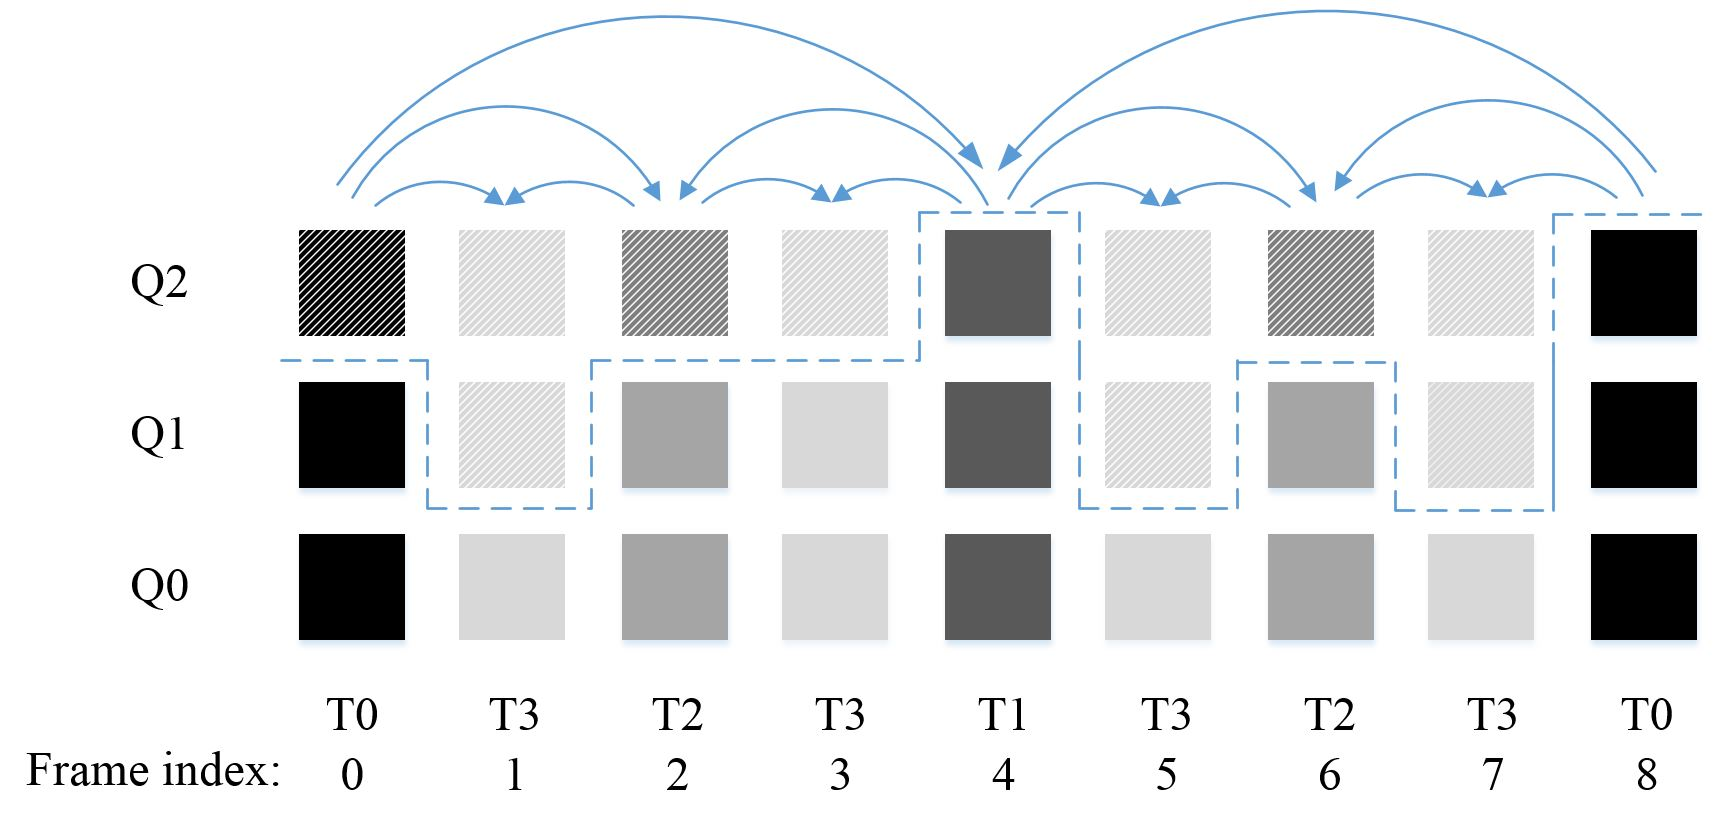
\includegraphics[width = 1.0\linewidth]{Bitstream-Extraction.jpg}
\caption{Bitstream extraction of SVC \label{fig:Bitstream-Extraction}}
\end{figure}

As we can see, in its nature SVC bitstream extraction is a combinatorial optimization problem. There are many combinations of packets to be discarded, and we want to choose a combination that maximizes the video quality of the extracted sub-stream, under the constraint of a given bitrate. More specifically, this problem fits in the form of ``0-1 Knapsack Problem" \cite{Knapsack}. Each data packet can be treated as an object with certain weight (the packet's size) and value (its contribution to the video quality). The solving process is mainly to decide whether or not a packet should be included in the final extracted sub-stream, or in the term of ``0-1 Knapsack Problem", to choose which object to pack up.

For a typical ``0-1 Knapsack Problem", the optimal solution can generally be found using the dynamic programming algorithm. However, this is not operational for the bitstream extraction problem, mainly due to the dependence between the stream's data packets. First, the subset of packets to be extracted cannot be chosen arbitrarily, since if a packet is included, all the packets it depends on must also be included. For example, in Fig. \ref{fig:Bitstream-Extraction}, we cannot include the Q2 packet of a frame without including the Q1 packet of the same frame. Second, the value of a packet is not obvious and certain, since a packet's contribution to video quality may depend on other packets. Unless we discard a packet and calculate the distortion it causes for real, there is no way to exactly tell its value. In fact, to the best of our knowledge, no method presented in the literature claims to find the optimal solution of the SVC bitstream extraction problem. All the effort is made to obtain a solution that is as good as possible.

In \cite{Amonou07}, Amonou et al. proposed a bitstream extraction framework based on the concept of \textit{Quality Layers}. This framework has been adopted by the SVC reference software, i.e., JSVM  \cite{JSVM}, and achieves better R-D performance compared with the basic extractor of JSVM. In Amonou's framework, a Quality Layer value, which reflects a packet's R-D impact, is calculated and used for R-D optimized bitstream extraction. The process of obtaining distortion impact of every packet is extremely time consuming, and the distortion estimation accuracy can also be further improved. So other distortion/error models were proposed to either reduce the computational complexity or improve the estimation accuracy. Sun et al. \cite{Sun09} and Maani et al. \cite{Maani09} constructed models to calculate distortion based on the drift propagation between frames. Sun et al.'s method is almost as good as JSVM in regard of performance, but has much reduced complexity. Maani et al.'s model can achieve better estimation accuracy than JSVM; however, since it is a training-based model, more computation is needed to get robust model parameters.
Ramanathan et al. \cite{Ramanathan12} proposed their concept and calculation method of the ``Quality Metadata'' to signal and use in bitstream extraction. Yang et al. \cite{Yang13} proposed a method based-on simulated annealing to solve the bitstream extraction problem. In both methods, the accuracy of distortion estimation is the key of the performance.

In our previous work \cite{Zhang12}, we noticed the mismatch between quadratic calculations in distortion criteria like MSE or PSNR and the essential linear operations in the coding process, and proposed a linear error model to directly estimate pixel value errors before MSE or PSNR is calculated. The linear error model exploits the linear feature of pixel value errors and achieves good performance in distortion estimation and bitstream extraction with reference. However, this work assumes that the original video sequence is available for reference, which is not always true. Adaptation to handle the special characteristic of the no-reference case is lacking in the previous work and included in this paper.

\subsection{Quality Control}

Quality control is the second problem we will address in this paper. The result of a quality control algorithm gives the suitable bitrate for current transmission, which is directly related to the change of video quality perceived by the user. In an SVC streaming system, the bitrate determined by the quality control algorithm is used as the constraint under which bitstream extraction is performed. Even in non-SVC streaming systems (DASH, for example), quality control is an important part that requires careful design.

For a quality control algorithm, there are three targets that should be achieved. First is to ensure the continuity of video playing. In real-time streaming system, each data packet has its own playtime, which is also regarded as the deadline of the transmission. If the packet does not arrive at client side before the deadline, the media player will be paused due to lack of data, and that should be avoided. The second is to keep a smooth video quality. Although network conditions may change rapidly, it is necessary for the streamed video to maintain a relatively stable quality level, since frequent change of video quality will lead to poor user experience. The third target is to make the video quality as good as possible. In other words, the available bandwidth should be fully utilized. Suppose we keep sending video data in a low bitrate (with low video quality as well), neither the playback will pause nor any quality fluctuation will happen. However, a low video quality is certainly not what we want.

The state-of-the-art solutions to avoid video pause in client media player mainly focus on how to select and schedule the video packets. In \cite{Gao06}, K. Gao et al. proposed a priority based scheduling strategy which guarantees packets of higher importance will be transmitted earlier. Among the packets with the same priority, those having the earliest deadline will be transmitted first. A similar solution is proposed in \cite{Schierl10}, where video data is pre-buffered in several buffers of different priorities. Whenever re-buffering occurs, quality will be degraded to a lower level to meet the time and rate constraint. Although the priority based scheduling strategies perform well in maintaining a non-paused video playing, they do not take quality fluctuation into account. As a result, users may still suffer from the frequent fluctuation of video quality.

In the widely-used video streaming server DSS, quality control is implemented by monitoring packet delay (the difference between current time and the playing time of this packet). When a new packet is ready to be sent to streaming buffer, DSS checks the delay of it and compares this delay with some pre-set thresholds to judge whether and how violently the quality change should be made. This algorithm can reduce quality fluctuation to some degree. However, it only provides conservative quality change, which makes its reaction so slow that sometimes media player may have already stopped due to lack of video data before quality drops. Furthermore, this algorithm does not keep track of the bandwidth change so it cannot adjust the video quality accordingly. Quality oscillation might occur in this algorithm.

The following of this paper will present our solution for each of the problems in detail. The solutions then work together and serve as a solid foundation for a practical adaptive video streaming system.


%%%%%%%%%%%%%%%%%%%%%%%%%%%%%%%%%%%%%%%%%%%%%%%%%%%%%%%%%%%%%
\section{Optimized Bitstream Extraction Based on Linear Error Model}
\label{sec:bitstream-extraction}

Being able to adjust bitrate is the prerequisite of an adaptive video streaming system. For SVC videos, it means to extract a subset of packets from the whole bitstream. How to optimally choose this subset to achieve minimum distortion under the given bitrate is the key point of bitstream extraction problem. In this section, we propose a linear error mode and a greedy-like algorithm to solve this problem.

\subsection{Linear Error Model for Quality Scalable Video}
\label{sec:model}

In H.264/AVC, the decoding process involves a linear feature described in \cite{Winken08}, neglecting any rounding, clipping, and deblocking filtering operation. According to this feature, the main steps in H.264/AVC coding -- prediction, transform and quantization -- are proximately linear operations, and the whole coding process can be expressed in a matrix format as follows:
\begin{equation}
\label{eq:linear}
s = {\rm\bf M} \cdot s + {\rm\bf T} \cdot c + p \: ,
\end{equation}
It means, the reconstructed samples of a GOP (Group of Pictures), denoted by $s$, can be viewed as a linear combination of previously reconstructed samples in the GOP, the residual samples, and a static predictor. In (\ref{eq:linear}), $c$ refers to the transform coefficient values and $p$ is a static predictor; ${\rm\bf M}$ and ${\rm\bf T}$ are square matrices such that the product ${\rm\bf M} \cdot s$ gives the MCP (Motion Compensated Prediction) signal and ${\rm\bf T} \cdot c$ gives the residual values. The actual values of ${\rm\bf M}$ depend on the selected macroblock types, reference indices and motion vectors, whereas the actual values of ${\rm\bf T}$ depend on the chosen QP (Quantization Parameter) values.

We apply the above linear decoding model to the case of quality scalability of SVC and get a Linear Error Model (LEM). According to (\ref{eq:linear}), for a bitstream just containing the base layer, we have:
\begin{equation}
\label{eq:base0}
s_{B} = {\rm\bf M} \cdot s_{B} + {\rm\bf T}_{B} \cdot c_{B} + p \: ,
\end{equation}
where the subscript $B$ indicates the base layer variables. In quality scalability, the enhancement is mainly the refinement of transform coefficients, so for a bitstream containing an enhancement packet set $I_1$, the reconstruction relationship can be expressed as:
\begin{equation}
\label{eq:subset1}
s_{I_1} = {\rm\bf M} \cdot s_{I_1} + {\rm\bf T}_{B} \cdot c_{B} + \Big( \sum_{i \in I_1}{\rm\bf T}_i \cdot c_i \Big) + p \: ,
\end{equation}
where $i$ refers to an enhancement packet as an element of $I_1$. $c_i$ is a vector containing coefficients within the enhancement packet $i$. ${\rm\bf T_i}$ is the transform matrix depending on the QP value of $i$. ${\rm\bf T}_i \cdot c_i$ gives the residual sample values decoded from $i$.

Similarly, for another bitstream containing an enhancement packet set $I_2$, we have
\begin{equation}
\label{eq:subset2}
s_{I_2} = {\rm\bf M} \cdot s_{I_2} + {\rm\bf T}_{B} \cdot c_{B} + \Big( \sum_{i \in I_2}{\rm\bf T}_i \cdot c_i \Big) + p \: .
\end{equation}

Suppose $I_1$ is a subset of $I_2$, their reconstruction difference can be obtained by (\ref{eq:subset2}) - (\ref{eq:subset1}):
\begin{equation}
\label{eq:minus1}
(s_{I_2} - s_{I_1}) = {\rm\bf M} \cdot (s_{I_2} - s_{I_1}) + \Big( \sum_{i \in I_2}{\rm\bf T}_i \cdot c_i - \sum_{i \in I_1}{\rm\bf T}_i \cdot c_i \Big) \: ,
\end{equation}
\begin{equation}
\label{eq:minus2}
\Rightarrow e = s_{I_2} - s_{I_1} = ({\rm\bf I - M})^{-1} \cdot \Big( \sum_{i \in I_2}{\rm\bf T}_i \cdot c_i - \sum_{i \in I_1}{\rm\bf T}_i \cdot c_i \Big) \: .
\end{equation}
	
Particularly, if the difference of $I_2$ and $I_1$ is a single enhancement packet $j$, i.e. $I_2 \setminus I_1 = \{j\}$, then according to (\ref{eq:minus2}), the difference of the two reconstruction vectors can be written as
\begin{equation}
\label{eq:error_j}
e_j = ({\rm\bf I - M})^{-1} \cdot {\rm\bf T}_j \cdot c_j \: .
\end{equation}
	
Obviously, $e_j$ is only determined by packet $j$, and has no relation with other enhancement packets. This value is called the ``error vector'' of packet $j$, which represents the pixel value error caused by discarding the packet $j$. We can obtain the error vector of each enhancement packet by subtraction between video sequences reconstructed from two enhancement packet subsets $I_1$ and $I_2$, with $I_1 \subseteq I_2$ and $I_2 \setminus I_1 =\{j\} $. Once all packets' error vectors are obtained, the distortion caused by discarding a group of packets can be estimated by adding up the error vector of each packet in the group.

Note that in equations (\ref{eq:base0})-(\ref{eq:subset2}) the value of ${\rm\bf M}$ and $p$ remain the same, since in the case of quality scalability the enhancement packets are generated only by manipulating the transform coefficients, and not interfered with the motion compensation and static prediction. This argument no longer holds for the other scalable dimensions (e.g., spatial scalability), so LEM does not simply apply for those cases. Therefore, only quality scalable videos are used in our system, and further research for other scalable dimensions can be our future work.

\subsection{Error Vector Acquisition}

It would need too many decoding times to get the error vectors of all enhancement packets if we calculate them one at a time. In order to acquire error vectors of all enhancement packets efficiently, we separate all enhancement packets into several groups, such that in each group multiple error vectors can be obtained independently at the same time.
 
\begin{figure}[h]
\centering
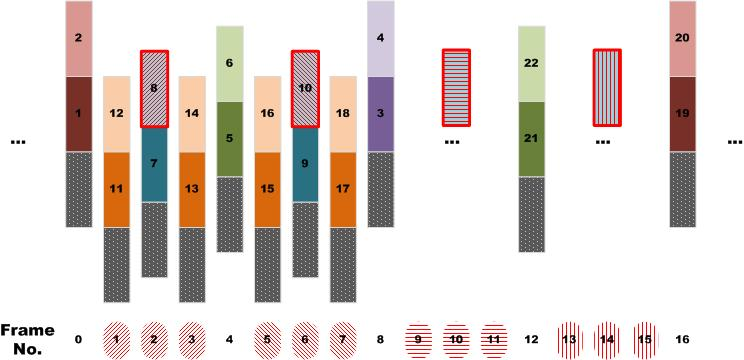
\includegraphics[width = 1.0\linewidth]{GOPStructure.jpg}
\caption{Group of pictures (GOP) in SVC \label{fig:GOP_Structure}}
\end{figure}
 
Consider a video bitstream with 8-frame GOPs shown in Fig. \ref{fig:GOP_Structure}. Base layer packets are colored black, and enhancement packets with the same color are allocated in one group. In each group, the enhancement packets' error vectors can be calculated simultaneously, since the pixel errors they caused are not interfered with each other. For example, the loss of packet 8 would bring about distortion only in frame 1, 2 and 3, while packet 10 only in frame 5, 6 and 7(frame number starts from 0). So we can do subtraction for this group, for one time, to gain error vectors $e_{8}$ and $e_{10}$, for both packets 8 and 10, as well as peer packets in all other GOPs. Note that these error vectors are highly sparse ones, because the discarding of a single enhancement packet can bring distortion only to a limited number of frames. To acquire all error vectors, the number of required extraction and decoding is approximately the number of enhancement layers $(L_Q - 1)$ times the temporal layer number $L_T$. For the example in Fig. \ref{fig:GOP_Structure}, $L_Q = 3$ and $L_T = 4$, so the theoretical extraction-and-decoding number is $(3 - 1) \times 4 = 8$. However, we have to do the same manipulation for $L_Q - 1 = 2$ more times, to dissociate the distortion impact of ``key frame'' \cite{H264Overview} (e.g. frame 0, 8, 16, etc.) packets. The loss of one enhancement packet in a key frame would bring distortion to two neighboring GOPs. As an instance, the loss of packet 4 would propagate drift into frame 1 to 15, which would interfere with the distortion impact of packets in frame 0 and 16 (packet 1, 2 and 19, 20). So key frame enhancement packets within the same quality layer (e.g. packet 2, 4 and 20) should be allocated in two groups -- one for key frame packets of even number GOPs (packet 2 and 20), the other for those of odd number GOPs (packet 4). Therefore, the actual number of extraction and decoding for error vector acquisition is $(L_Q - 1) \cdot (L_T + 1)$, approximately the same with the Quality Layer information acquisition in JSVM \cite{Amonou07}. Since computation is mainly consumed with this decoding in the bitstream extraction algorithm, the computation complexity has no obvious promotion compared with JSVM.
 
\subsection{Distortion Estimation and Model Verification}

Based on the linear error model described above, we can obtain error vectors of all enhancement packets. Then we can estimate the distortion caused by discarding any set of enhancement packets, by adding up the error vector of each packet in that set.

For example, consider a video sequence decoded from a sub-stream which is extracted by discarding packet set $I_x$. The error between this sequence and the original sequence can be estimated as
\begin{equation}
\label{eq:subset_error}
e(I_x) = e_{full} + \sum_{i \in {I_x}} e_i \: .
\end{equation}
Eq. (\ref{eq:subset_error}) has taken into consideration the error between the video sequence decoded from full enhancement packets and the original sequence, written as $e_{full}$.

To verify the linear error model, we conduct an experiment where random combinations of enhancement packets are removed from a video bitstream, and the distortion estimated by the linear error model are compared with the actual distortion caused by the removal. The video stream has the same GOP structure and quality layers as illustrated in Fig. \ref{fig:GOP_Structure}. One comparison result for the sequence {\em Foreman} (only first 33 frames are used) is shown in Fig. \ref{fig:model_verification}. The horizontal axis stands for frame index, and the vertical axis for MSE measurement. The solid line represents the actual MSE of a frame, and the dot line shows the estimated MSE using our Linear Error Model. It can be seen that the two lines are very close to each other, which demonstrates the accuracy of the proposed model. Table \ref{tab:estimation-error} lists the distortion estimation error for different sequences and shows that the average error is only about 5\%.

\begin{figure}[h]
\centering
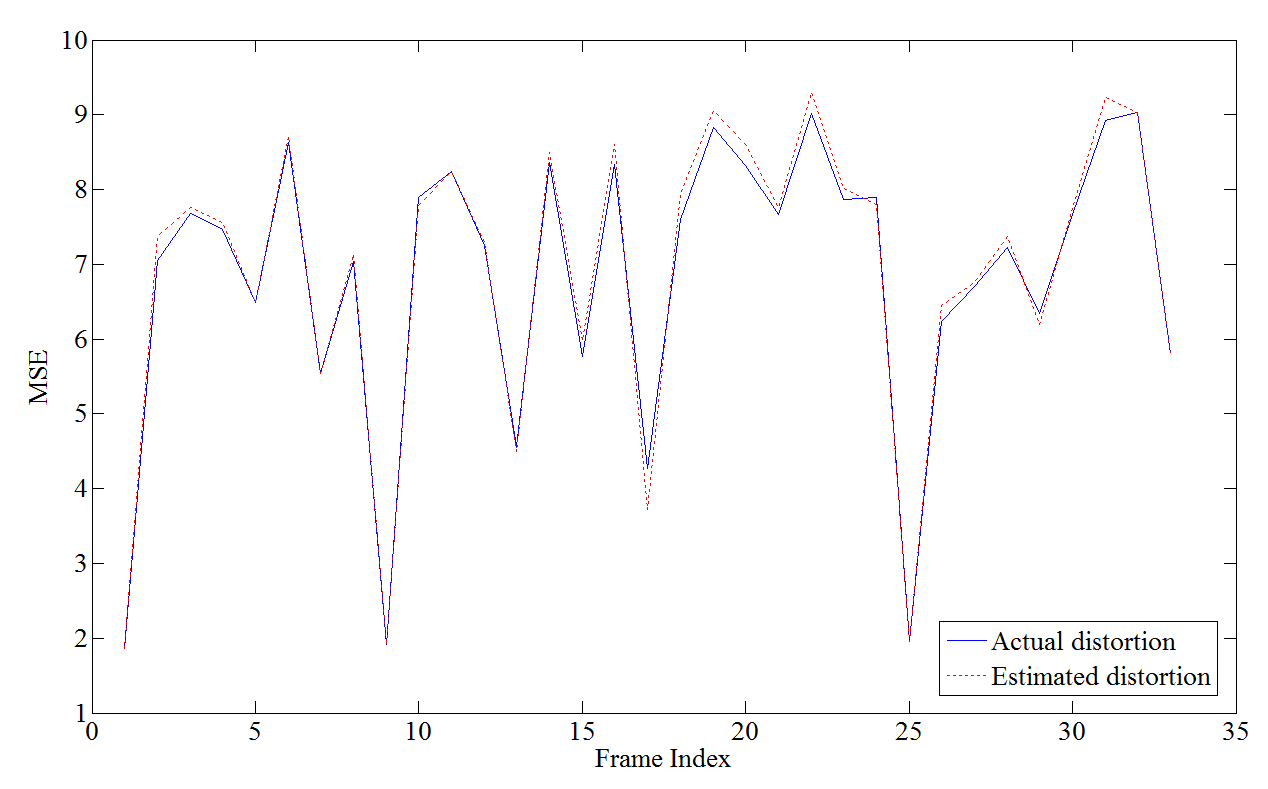
\includegraphics[width = 1.0\linewidth]{ModelVerification.png}
\caption{Comparison of actual and estimated distortion for sequence {\em Foreman} \label{fig:model_verification}}
\end{figure}

\begin{table*}
\centering
\caption{Performance of distortion estimation using LEM}
\label{tab:estimation-error}
\begin{tabular}{c|*{8}{p{1.2cm}<{\centering}|}{p{1.2cm}<{\centering}}}
	\hline\hline
	Sequence name & {\em Bus} & {\em City} & {\em Crew} & {\em Football} & {\em Foreman} & {\em Harbour} & {\em Mobile} & {\em Soccer} & \textbf{Average} \\ \hline
	Estimation error  & 2.83\% & 2.39\% & 10.36\% & 7.08\% & 4.95\% & 2.63\% & 5.77\% & 5.26\% & \textbf{5.16\%} \\ \hline
\end{tabular}
\end{table*}

\subsection{Priority Assignment and Bitstream Extraction}
\label{subsec:priority}

In this subsection, we utilize the linear error model to enable R-D optimized bitstream extraction. Since finding the global optimal solution of the bitstream extraction problem is impractical, our bitstream extraction algorithm uses a greedy method \cite{GreedyAlgo} to get a sub-optimal solution. Similar to the greedy solution of the ``0-1 Knapsack Problem", every time a packet is to be discarded, we choose the packet that has the minimal R-D impact. A packet's R-D impact is mathematically measured by:
\begin{equation}
\label{eq:rd_impact}
\Phi_{i} = \dfrac{\partial D}{\partial R} \: ,
\end{equation}
where $\partial D$ represents the distortion change brought by discarding this packet, and $\partial R$ is the corresponding rate change. $\partial R$ is simply equivalent to the size of this packet, while $\partial D$ needs to be calculated by subtraction of distortions before and after the packet is discarded.

We simulate a process of discarding all the enhancement packets from a stream, using the above greedy strategy. During this process, the discarding order of a packet is regarded as its priority and recorded. Then the packets' priority values can be stored in the bitstream (either in the priority identifier field of the NALU header or in supplementary enhancement information messages) for real extraction in the future.

The detailed discarding and priority assignment process is described below:
\begin{description}
\item[1)] Initially, the sequence error vector, $e_{seq}$, is set to $e_{full}$.
\item[2)] Within the packets that can be discarded, find the packet $m$ having the least RD impact on the sequence, \textit{i.e. }
\begin{equation}
\label{eq:R-D_impact_m}
\Phi_m = \min_{i \in I_{top}} \Phi_i \: ,
\end{equation}
where $I_{top}$ stands for the top-layer packets, those currently able to be discarded. The RD impact of a packet is calculated based on (\ref{eq:rd_impact}), as follows: 
\begin{equation}
\label{eq:R-D_impact_i}
\Phi_i = \dfrac{\partial D}{\partial R} = \dfrac{PSNR(e_{seq}) - PSNR(e_{seq} + e_i)}{SIZE(i)} \: ,
\end{equation}
where $PSNR(*)$ means to obtain PSNR from the error vector, and $SIZE(i)$ is the size of packet $i$.
\item[3)]The packet, $m$, is then removed from the bitstream, and its error vector is added to the sequence's error vector, \textit{i.e.}
\begin{equation}
\label{eq:error_update}
e_{seq} = e_{seq} + e_m \: .
\end{equation}
\item[4)]The process from 2) to 3) is repeated until all enhancement packets are discarded, and every packet is assigned a priority value according to the removing order.
\end{description}

For long video sequences, an optimization window containing a certain number of frames is usually needed, and the priority assignment and bitstream extraction is conducted independently in each window. Suppose the size of the optimization window is $K$, i.e., there are $K$ frames involved in the above priority assignment process, and each frame contains $L_Q$ quality layers (one base layer and $L_Q-1$ enhancement layers). Then the number of top layer packets in step 2) of the process is $K$, and the total number of packets that can be discarded is $K \cdot (L_Q-1)$. Given that, the priority assignment process in each optimization window can be more specifically described in Algorithm \ref{algo:greedy}. It is easy to see that the computational complexity of this priority assignment algorithm is $O(K^2)$. Note that this computational complexity is negligible compared with the decoding process needed in the error vector acquisition.

\begin{algorithm}
\caption{Greedy-like bitstream extraction algorithm}
\label{algo:greedy}
\begin{algorithmic}
    \STATE Set $e_{seq}$ to $e_{full}$, and set $p$ to 0.
    \WHILE{$p < K \cdot (L_Q - 1)$}
	    \FOR{$K$ top layer packets}
		    \STATE Find the packet $m$ which has least RD impact
		\ENDFOR
		\STATE Set the priority value of packet $m$ to $p$
		\STATE Remove $m$ from the sequence
		\STATE Set $e_{seq}$ to $e_{seq} + e_m$, and set $p$ to $p+1$
    \ENDWHILE
\end{algorithmic}
\end{algorithm}

A larger optimization window means each time we have more packets to compare and determine their priorities. Therefore, choosing a larger $K$ will result in more optimized extraction. However, doing this will also increase the computational complexity as well as the memory used to store the error vectors. Besides, if the 6-bit priority identifier field of the NALU header is used to store the priority values, only a range of 0$\sim$63 is supported, which also limits the value of $K$.

\subsection{The No-Reference Case}
\label{subsec:noref}

In some scenarios, the priority assignment and bitstream extraction needs to be conducted without access to the original YUV sequence. For example, if the bitstream extraction is not done at the encoding side, it's most likely that the original sequence is not available. This would make the bitstream extraction a more difficult problem, since the distortion is harder to obtain for lacking of reference signal. Comparing to the problem of SVC bitstream extraction with reference, this kind of ``no-reference bitstream extraction'' problem is actually more frequently encountered in real practice. In this subsection, we consider this no-reference problem and modify the proposed algorithm to meet the special characteristic caused by lacking of reference.

In the no-reference case, since we do not have access to the original sequence, we can not get the error between the video sequence decoded from full enhancement packets and the original sequence, which is $e_{full}$ used above. A straightforward idea is to set $e_{full}$ to zero, meaning we calculate distortion with respect to the fully reconstructed signal, rather than to the original sequence. However, simply doing so causes the algorithm to perform badly in experiments. We find that, since discarding some enhancement packets will not bring much significant error relative to the fully reconstructed signal, the calculated PSNR values are too large to well represent the real distortion. To address this issue, instead of calculating PSNR, we directly use MSE of all pixels as the distortion criteria in the priority assignment algorithm. This proves to be an effective solution, and the extraction performance turns out to be much better.

After each packet is assigned a priority value and optimized extraction is made possible, the video stream now can well adapt to different data rates. Next, we propose the quality control algorithm based on the PID mechanism, which is responsible for determining a suitable data rate according to current bandwidth condition.

%%%%%%%%%%%%%%%%%%%%%%%%%%%%%%%%%%%%%%%%%%%%%%%%%%%%%%%%%%%%%
\section{PID-based Quality Control Algorithm}
\label{sec:quality-control}

PID control \cite{PID}\cite{Astrom02} is a control loop feedback mechanism commonly used in industrial control systems. \textit{Process variable} and \textit{setpoint} are two core concepts in PID control. The process variable stands for the current status of the system. The setpoint is the target for this automatic control system to reach. The goal of PID control is to minimize the error between process variable and setpoint by adjusting system inputs. The controller output $u(t)$ is defined as follows:

\begin{equation}
\label{eq:pid-output}
u(t) = {K_p} \cdot e(t) + {K_i} \cdot \int_0^t {e(\tau )d\tau }  + {K_d} \cdot \frac{d}{{dt}}e(t) \: ,
\end{equation}
where $e(t)$ represents the error between process variable and setpoint at time $t$. $K_p$, $K_i$, and $K_d$ here are tuning parameters representing the proportional gain, integral gain and derivative gain respectively. Proportional part directly relates to the change of the process variable, and is also the main factor to adjust the process variable towards setpoint. There might be oscillations and steady-state errors in a pure proportional system, and they can be reduced or eliminated by adding the integral part. The appearance of derivative part is to predict future errors, so that the system tends to become steady early and quickly. The result of (\ref{eq:pid-output}) is used to manipulate the system input of next moment to adjust process variable towards setpoint.

As an effective and flexible control technique, PID control has been used to solve all kinds of control problems. In the area of video coding, we notice that PID is utilized to design rate control algorithms by many papers. For instance, in \cite{Wong04} a PID-based real time rate control scheme is proposed to trade-off between spatial and temporal quality and smooth the video quality between frames; in \cite{Yang10}, the authors designed an incremental rate control algorithm for H.264/SVC, in which the PID method is used to provide robust buffer control for each layer. We also notice that some researchers have proposed theoretical model or middle-ware framework for QoS adaptation \cite{Li98}\cite{Li99}, with PID as the basic control concept. However, we have not found any paper that integrates PID method into the quality control of video streaming. While rate control of video coding and quality control of video streaming are two different problems, they do share some common properties, such as the buffer mechanism and the requirement for smoothness. That inspires us to design a PID-based quality control algorithm and utilize it to deliver best video quality with least quality fluctuation.

In this section, we first introduce the \textit{quality level} concept to discretization the bitrate and quality of scalable video. Then we define the process variable used in our PID-based quality control algorithm. After that, the algorithm is formulated and explained in detail, followed by the brief discussion of parameter selection.

\subsection{Quality Level}
\label{subsec:quality-level}

The video quality is a continuous value. In practical operation, it is not possible to control it at an arbitrary precision. So we propose a \textit{quality level} concept as the discrete description of the video quality. When the video quality needs to be adjusted, we simply increase or decrease the quality level. Each quality level corresponds to a certain bitrate. A higher quality level corresponds to a higher bitrate and vice versa. The number of quality levels and how they are mapped to sub-streams with different bitrates depends on actual requirement or implementation. The more quality levels are defined, the more precisely the control algorithm can adjust bitrate to follow the bandwidth change. As pointed out in section \ref{sec:intro}, simulcast streaming systems can only have limited quality levels while SVC streaming systems can define quality levels at a much finer granularity.

\subsection{Process Variable Selection}
\label{subsec:variable}

In our PID-based quality control algorithm, the process variable is called \textit{actual\_check interval ratio}, which is defined as follows.

In DSS, two timelines are important. Push timeline indicates the time of pushing video data packets to streaming buffer, and play timeline indicates the time these data packet should be played, i.e., the presentation time stamp (often seen as PTS) of each packet. Their relationship is shown in Fig. \ref{fig:intervals}. The program will check the timelines periodically, and, in the default quality control algorithm of DSS, use the packet delays to decide whether quality change is needed. The two intervals shown in Fig. \ref{fig:intervals}, i.e., check interval and actual interval, are worth notice and may provide useful information. In the ideal situation, during each check interval, the server pushes an amount of data that will actually play for a period of time equal to that check interval, i.e., \textit{actual\_interval} = \textit{check\_interval}. If \textit{actual\_interval} is smaller than \textit{check\_interval}, it means that less data is pushed to the client, and the pushing is slowed down because bandwidth is relatively low at this time. On the other hand, if \textit{actual\_interval} is larger than \textit{check\_interval}, it indicates the bandwidth condition is good and data is being pushed quickly to the client. The ratio of these two intervals, i.e., \textit{actual\_check interval ratio}, is in direct proportion to the ratio of the data rate appropriate for bandwidth and the current pushing data rate.

The \textit{actual\_check interval ratio} is suitable for quality control because: 1) this ratio directly reflects the mismatch of current pushing data rate and the bandwidth, and by adjusting data rate according to it, this ratio can be used to accurately change video quality; 2) the desired value of this ratio is 1.0 by definition so we don't need to find the optimized setpoint by mathematical methods or experiments; and 3) it is easy to compute and implement in practical systems.

\begin{figure}[t]
\centering
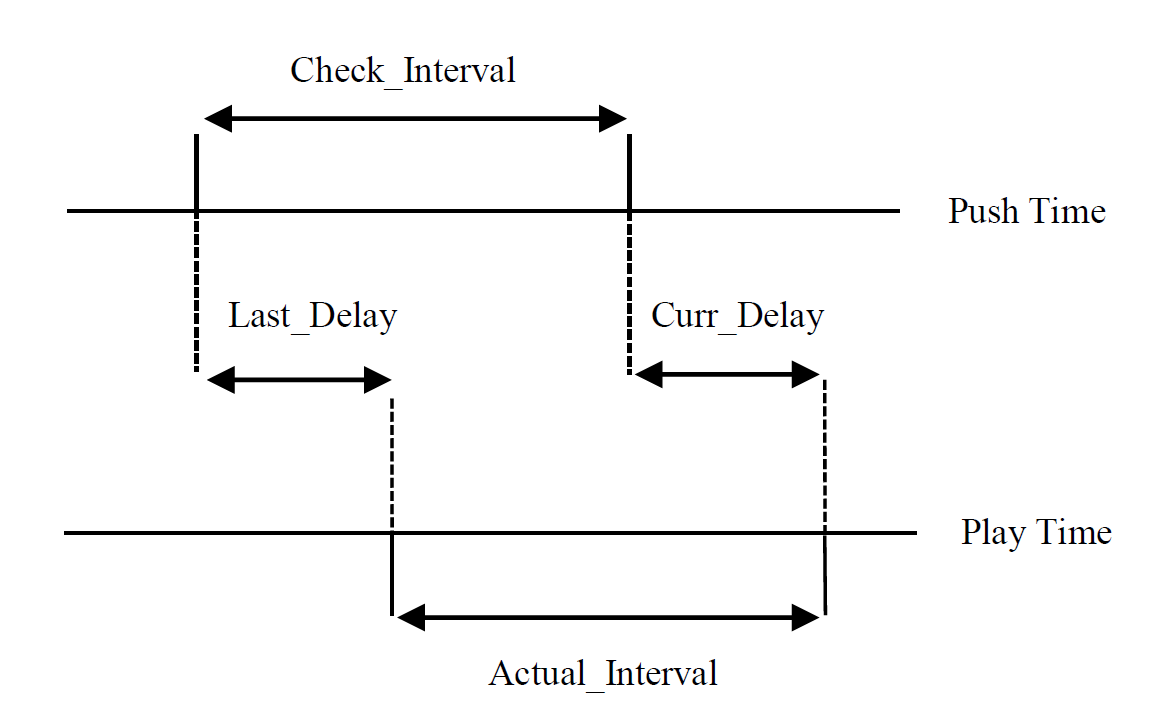
\includegraphics[width = 0.9\linewidth]{Intervals.jpg}
\caption{Two timelines in Darwin Streaming Sever (DSS) \label{fig:intervals}}
\end{figure}

\subsection{Model Formulation}
\label{subsec:model}

As is introduced above, the \textit{actual\_check interval ratio} serves as the process variable in this PID-based quality control algorithm. In normal PID control, the controller output is calculated using the proportion, integral and differential of the error between the process variable and the setpoint, as shown in (\ref{eq:pid-output}). Considering that the chosen process variable is a ratio and the corresponding setpoint is 1, we make a little modification to the general PID controller and obtain a ratio-based model. In this model, the ratio is directly used to calculate the controller output, and all subtraction operations in original PID equations have been changed to division operations to keep the correctness, as follows:

\begin{equation}
\label{eq:ut}
{u_t} = {K_p} \cdot E_p^t + {K_i} \cdot E_i^t + {K_d} \cdot E_d^t ,
\end{equation}

\begin{equation}
\label{eq:ep}
E_p^t = \frac{{actual\_interva{l_t}}}{{check\_interva{l_t}}} ,
\end{equation}

\begin{equation}
\label{eq:ei}
E_i^t = \frac{{long\_actual\_interva{l_t}}}{{long\_check\_interva{l_t}}} ,
\end{equation}

\begin{equation}
\label{eq:ed}
E_d^t = E_p^t/E_p^{t - 1} ,
\end{equation}

\begin{equation}
\label{eq:long-actual}
long\_actual\_interva{l_t} = \sum\limits_{\tau = {T_l}}^t {actual\_interva{l_\tau}} ,
\end{equation}

\begin{equation}
\label{eq:long-check}
long\_check\_interva{l_t} = \sum\limits_{\tau = {T_l}}^t {check\_interva{l_\tau}} .
\end{equation}


In (\ref{eq:ut}), $K_p$, $K_i$, and $K_d$ indicate the tuning parameters for proportional, integral and derivative parts respectively, and $E_p^t$, $E_i^t$, $E_d^t$ stand for the corresponding observed value for each part, which are defined in (\ref{eq:ep})-(\ref{eq:long-check}); the controller output $u_t$ is utilized to calculate an appropriate data rate and further to determine which quality level we should transmit (see Algorithm \ref{algo:control} for more details).

In (\ref{eq:long-actual}) and (\ref{eq:long-check}), $T_l$ stands for the last quality change time. Theoretically, the integral part should be recorded and calculated since the system starts. In practice, however, bandwidth may vary significantly during the transmission. If the integral part was recorded for too long time, it may not reflect the real network status and may slow down the reaction for better quality level. A compromise here is to choose a relatively long time, i.e., the time from last quality change till now, for the integral part calculation.

This ratio-based model is more simple and effective for the chosen process variable and setpoint. And note that, since the controller output ($u_t$) is also a ratio, it should be used as a multiplier to manipulate the system input, i.e., the pushing data rate.

The whole process of this algorithm is described in Algorithm \ref{algo:control}. Compared to other scheduling strategies, this quality control algorithm has several advantages. First, this algorithm does not just rely on current packet delay or information at fixed time point, so quality change may occur at any proper time. Second, since the model has taken prediction into account, we can actually decide whether the bandwidth will be high or low enough for the quality level to change, thus avoiding video quality fluctuation. Third, in this algorithm it's not necessary to change one quality level at a time. This enables fast quality drop when bandwidth suddenly decreases and fast quality rise when system starts, resulting in a seamless experience.

\begin{algorithm}
\caption{PID-based quality control algorithm}
\label{algo:control}
\begin{algorithmic}
    \STATE before packet sent
    \STATE check\_interval = curr\_time -- last\_check\_time
    \STATE actual\_interval = curr\_media\_time -- last\_check\_media\_time
    \STATE long\_check\_interval += check\_interval
    \STATE long\_actual\_interval += actual\_interval
    \STATE calculate $E_p^t$, $E_i^t$, $E_d^t$ according to Eq. (\ref{eq:ep}) - (\ref{eq:ed})
    \STATE output = ${K_p} \cdot E_p^t + {K_i} \cdot E_i^t + {K_d} \cdot E_d^t$
    \STATE new\_bitrate = output * curr\_bitrate
    \STATE new\_level = get\_level(new\_bitrate, bitrate\_of\_level[])
    \IF {quality level changed}
    	\STATE long\_check\_interval = 0
    	\STATE long\_actual\_interval = 0
    	\STATE curr\_bitrate = bitrate\_of\_level[new\_level]
    \ENDIF
    \STATE send packet according to new quality level
\end{algorithmic}
\end{algorithm}


\subsection{Parameter Selection}
\label{subsec:parameter}

Ziegler--Nichols method \cite{Ziegler42} is used to tune $K_p$, $K_i$, and $K_d$ to obtain better performance of the PID control system. This method is performed by setting integral and derivative parameters to zero and then tuning $K_p$ to a value $K_u$ until output begins to oscillate with constant amplitude. Assuming the oscillation period is $T_u$, we set $K_p = 0.6K_u$, $K_i = 2K_u/T_u$, and $K_d = K_u \cdot T_u/8$. $K_p$, $K_i$, and $K_d$ are then normalized to get the final parameters. In the following experiments, parameters are chosen as $K_p = 0.22$, $K_i = 0.73$, $K_d = 0.05$ by this method. As with other control systems, PID parameters are a result of tunning and may not suit to all use cases. However, it should be noted that in the video quality control algorithm, only the data rate and the bandwidth are considered, not the video content. Therefore once the parameters are tuned they should apply well to different video streams.


%%%%%%%%%%%%%%%%%%%%%%%%%%%%%%%%%%%%%%%%%%%%%%%%%%%%%%%%%%%%%
\section{Experimental Results}
\label{sec:experiment}

To implement our proposed adaptive streaming system requires the combination of the optimized bitstream extraction method and the PID-based quality control algorithm. The latter determines the current bitrate to follow the bandwidth change, and the former will ensure the sub-stream with the best possible quality is obtained and sent under that bitrate constraint. They work together to deliver best quality of service for the user. Choosing DSS as the implementation basis, we have integrated the proposed algorithms into it for the purpose of both research and application. In this section, we first present separate experiments to show the advantage of each proposed solution, and then give the result when they are combined together. Readers who are interested in the practical implementation and demonstration can visit the online video website http://www.7dlive.com for more information.

\subsection{Experiments for Bitstream Extraction}

We compare the performance of the proposed bitstream extraction method with that of JSVM 9.16.

In our experiments, all test bitstreams are encoded with the JSVM encoder, where the standard hierarchical B coding structure and CABAC entropy coding are used. Each bitstream contains one base layer and a quality enhancement layer, with quantization parameters QP = 33 and QP = 27, respectively. The enhancement layer is further divided into 2 MGS layers by configuring the MGS vector to separate the transform coefficients into two groups (containing 4 and 12 coefficients respectively). For each test bitstream, ten bitrate points (one with all enhancement packets, one with only the base layer packets, and 8 points between) are chosen for extraction. For each bitrate point, the extraction is conducted using the bitstream extractors in JSVM, with and without quality layer (denoted as JSVM QL and JSVM Basic, respectively), and the proposed method. The size of the optimization window in the proposed method is set to 4 GOPs, with a GOP size of 8. All of the eight SVC standard sequences with CIF resolution are considered at 30FPS and tested in our experiments.

The performance comparisons for City, Foreman, Harbour, and Soccer are shown in Fig. \ref{fig:performance}. It can be seen that the R-D curves of the proposed method are always on the top. For each sequence, the maximum and average PSNR gain through all 10 bitrate points are calculated and listed in Table \ref{tab:results}, which shows that our extraction method can achieve a significant performance gain compared with JSVM.

Among other bitstream extraction methods besides that of JSVM, the work in \cite{Maani09} achieves much better performance than JSVM QL, and even better than ours. However, the method of \cite{Maani09} needs more computation in order to train robust model parameters for different sequences, while the complexity of our method is always the same with JSVM QL.

\begin{figure*}[t]
\centering
\subfloat[City]{
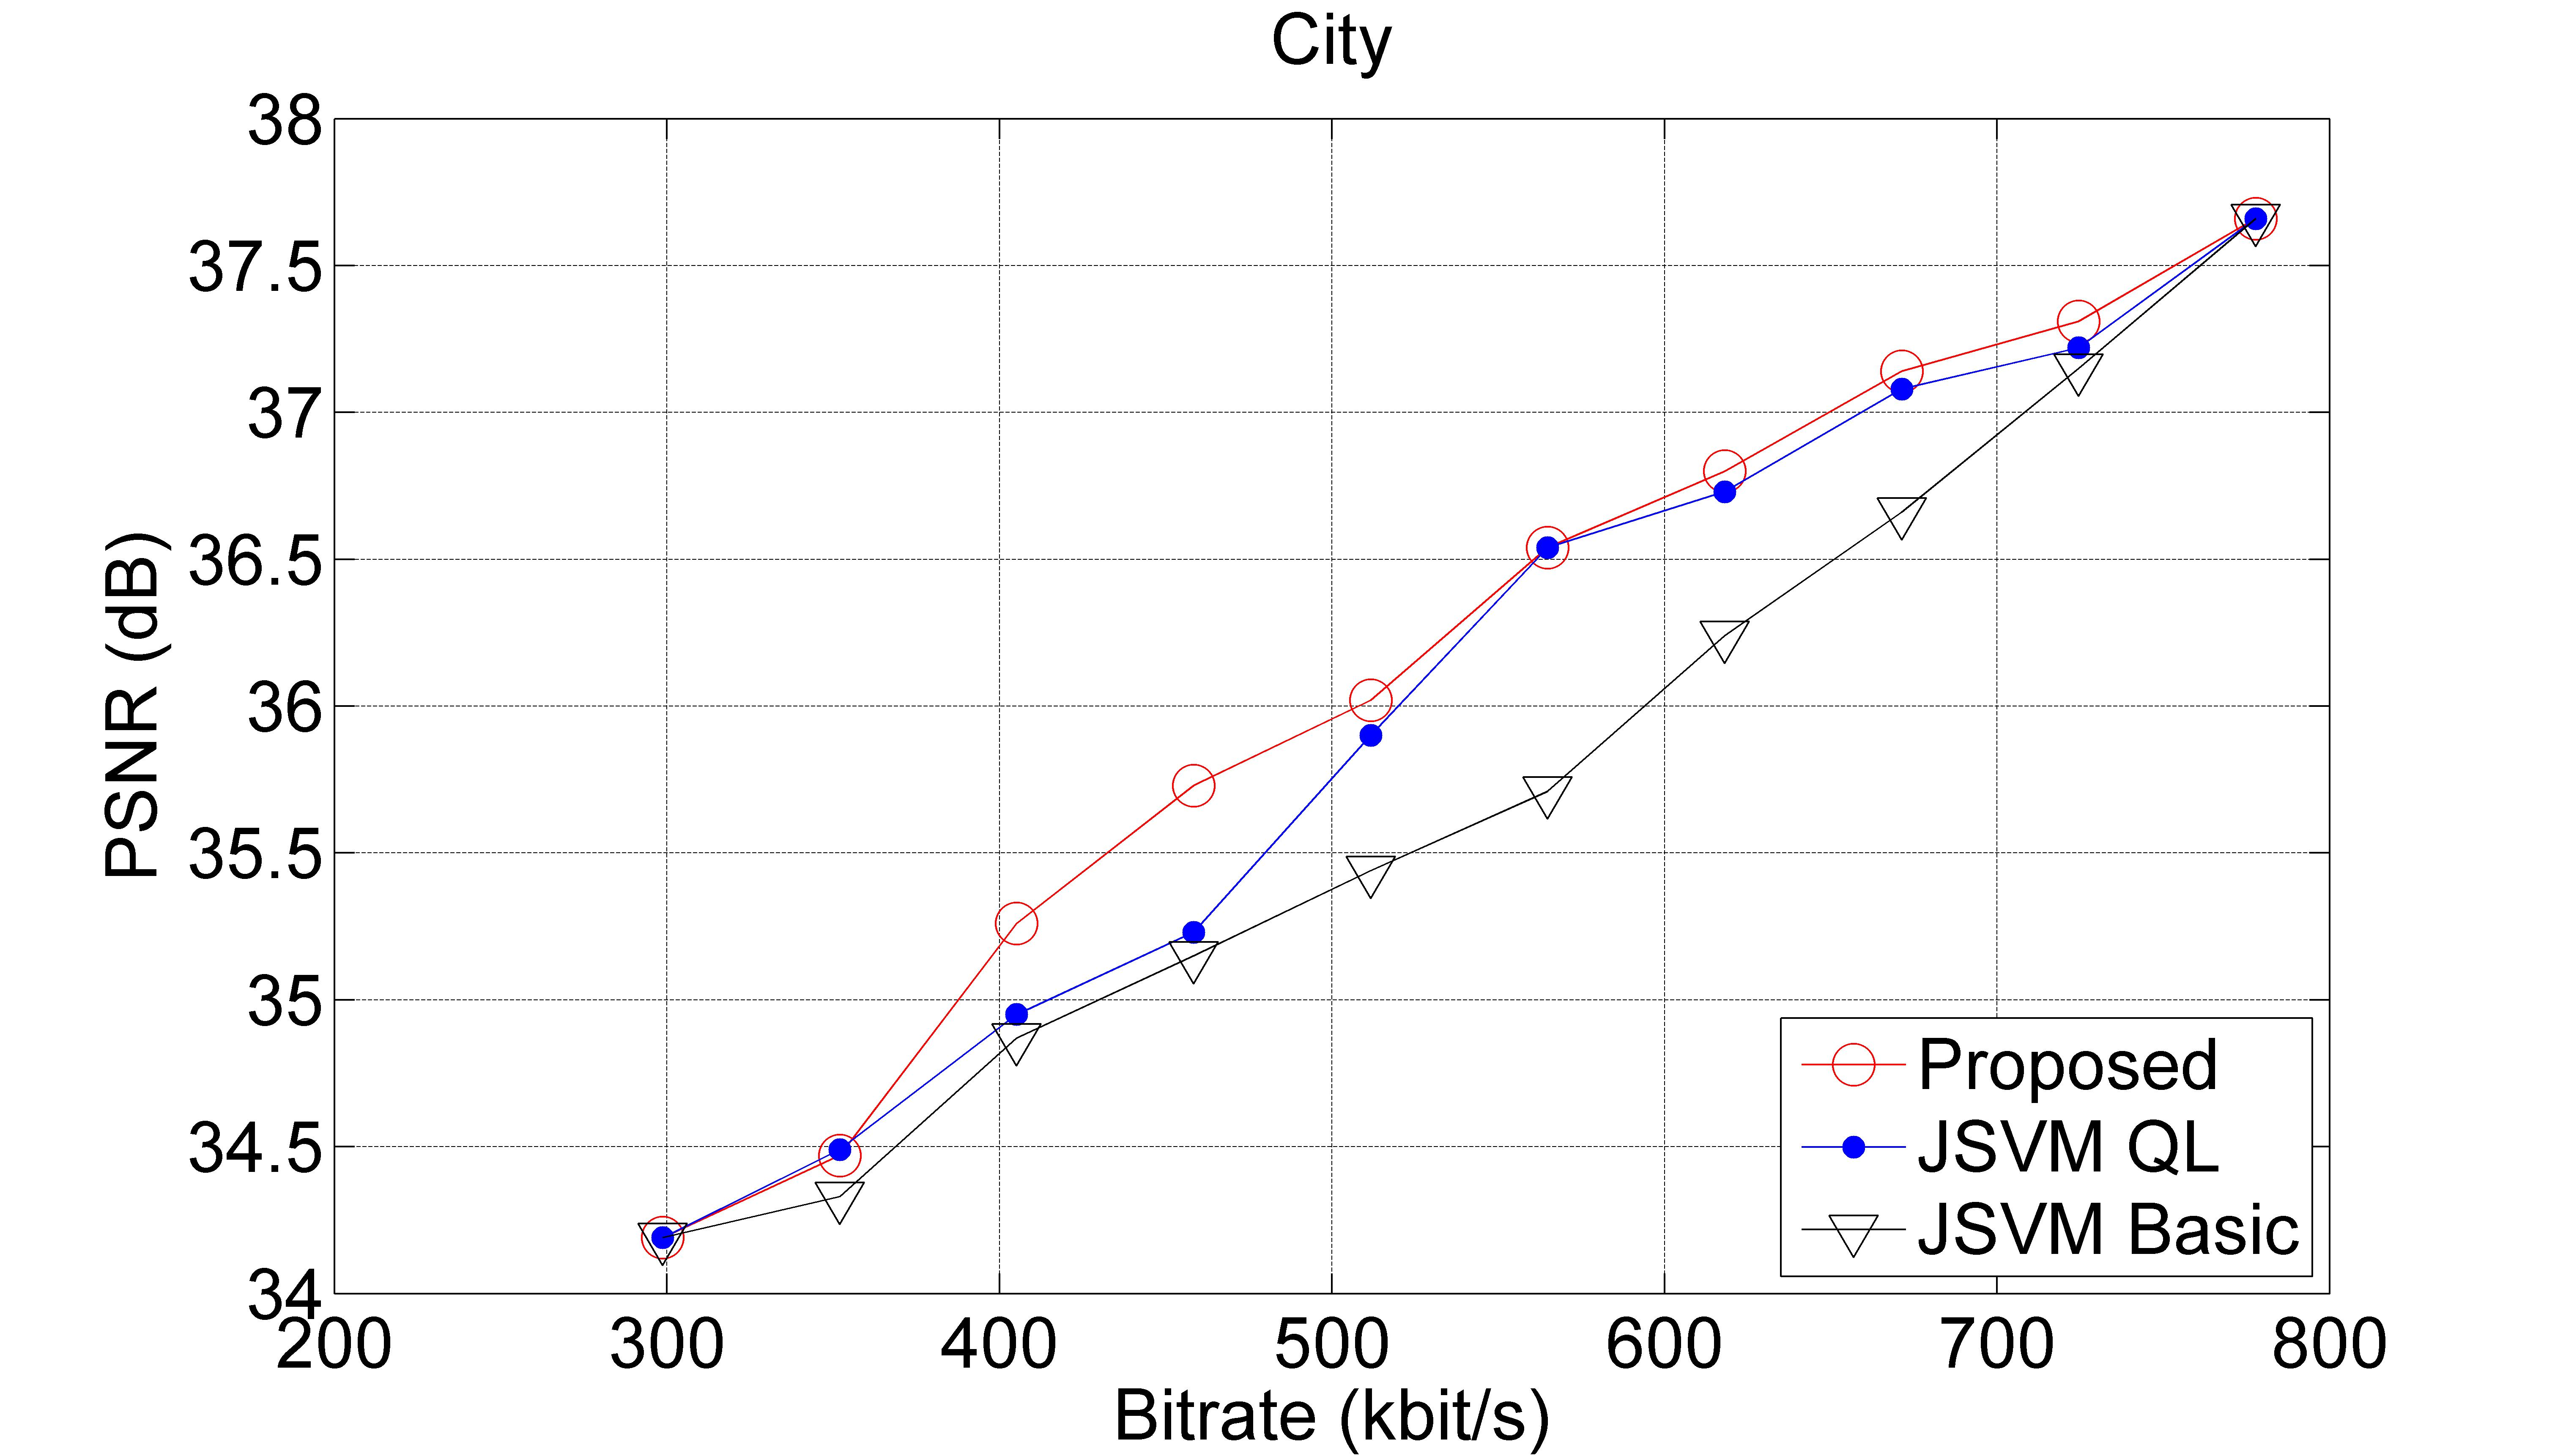
\includegraphics[width=0.5\textwidth]{City.jpg}
\label{fig:City}}
\subfloat[Foreman]{
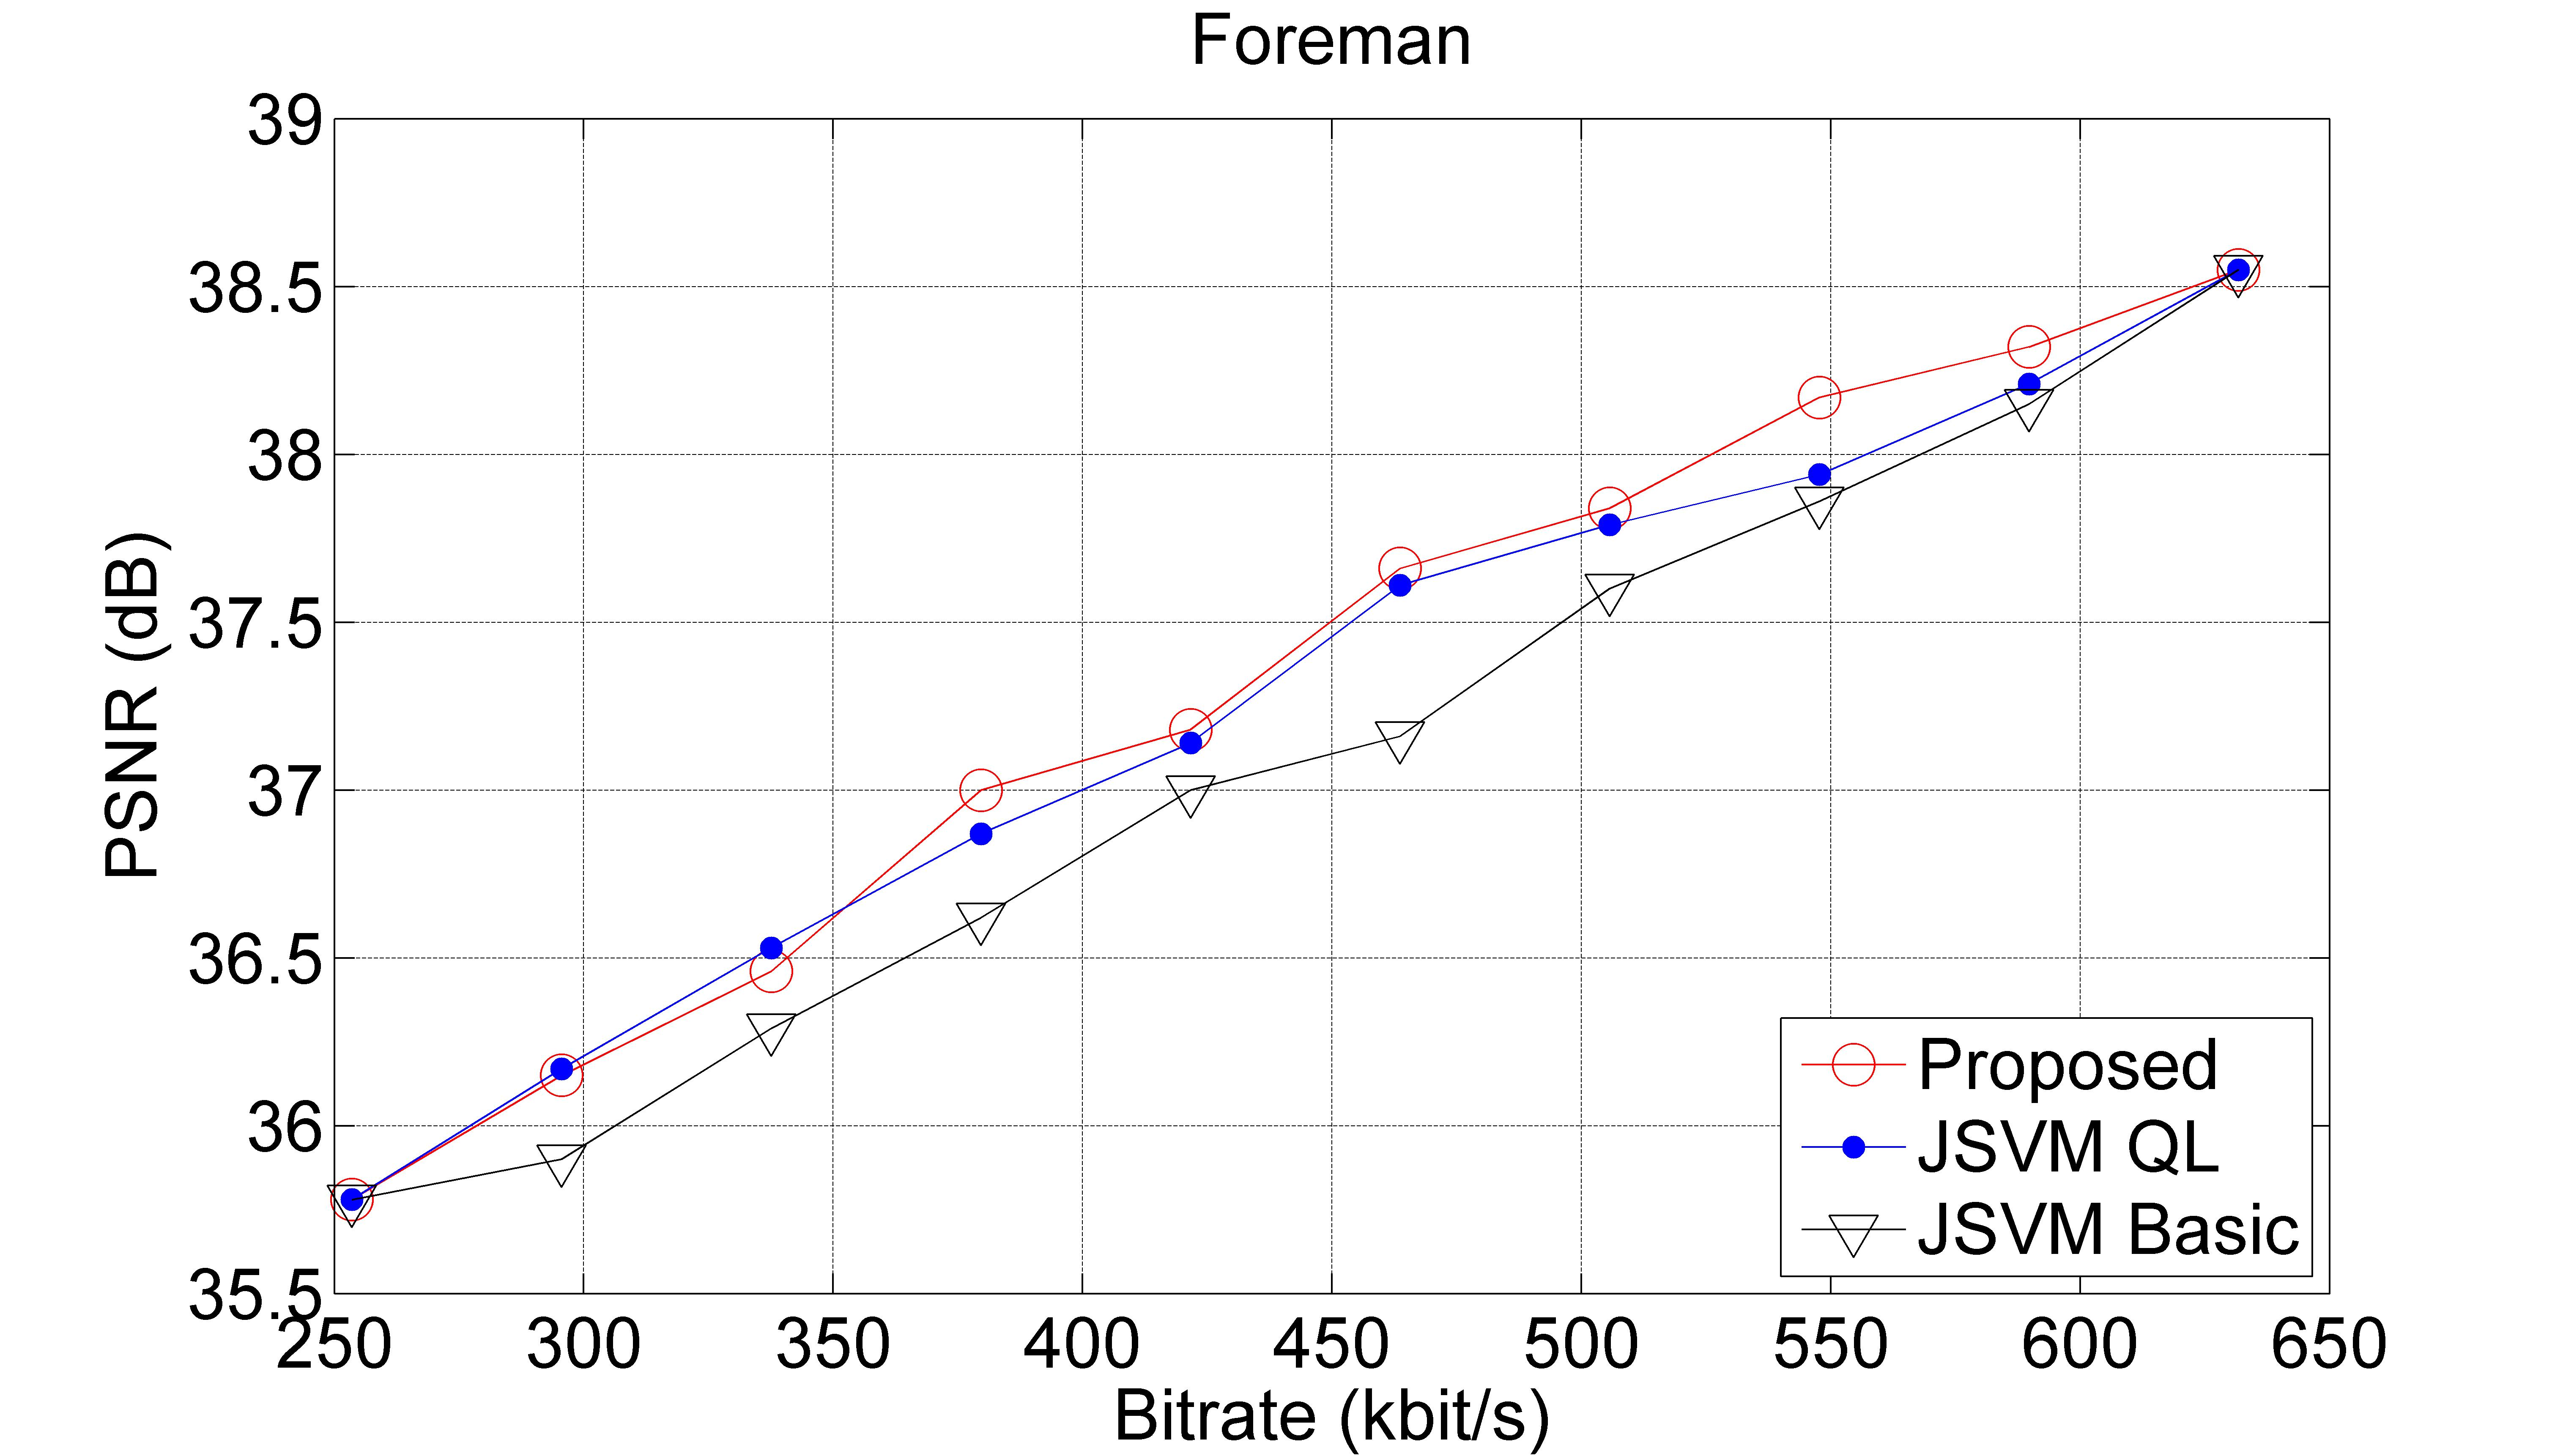
\includegraphics[width=0.5\textwidth]{Foreman.jpg}
\label{fig:Foreman}}
\qquad
\subfloat[Harbour]{
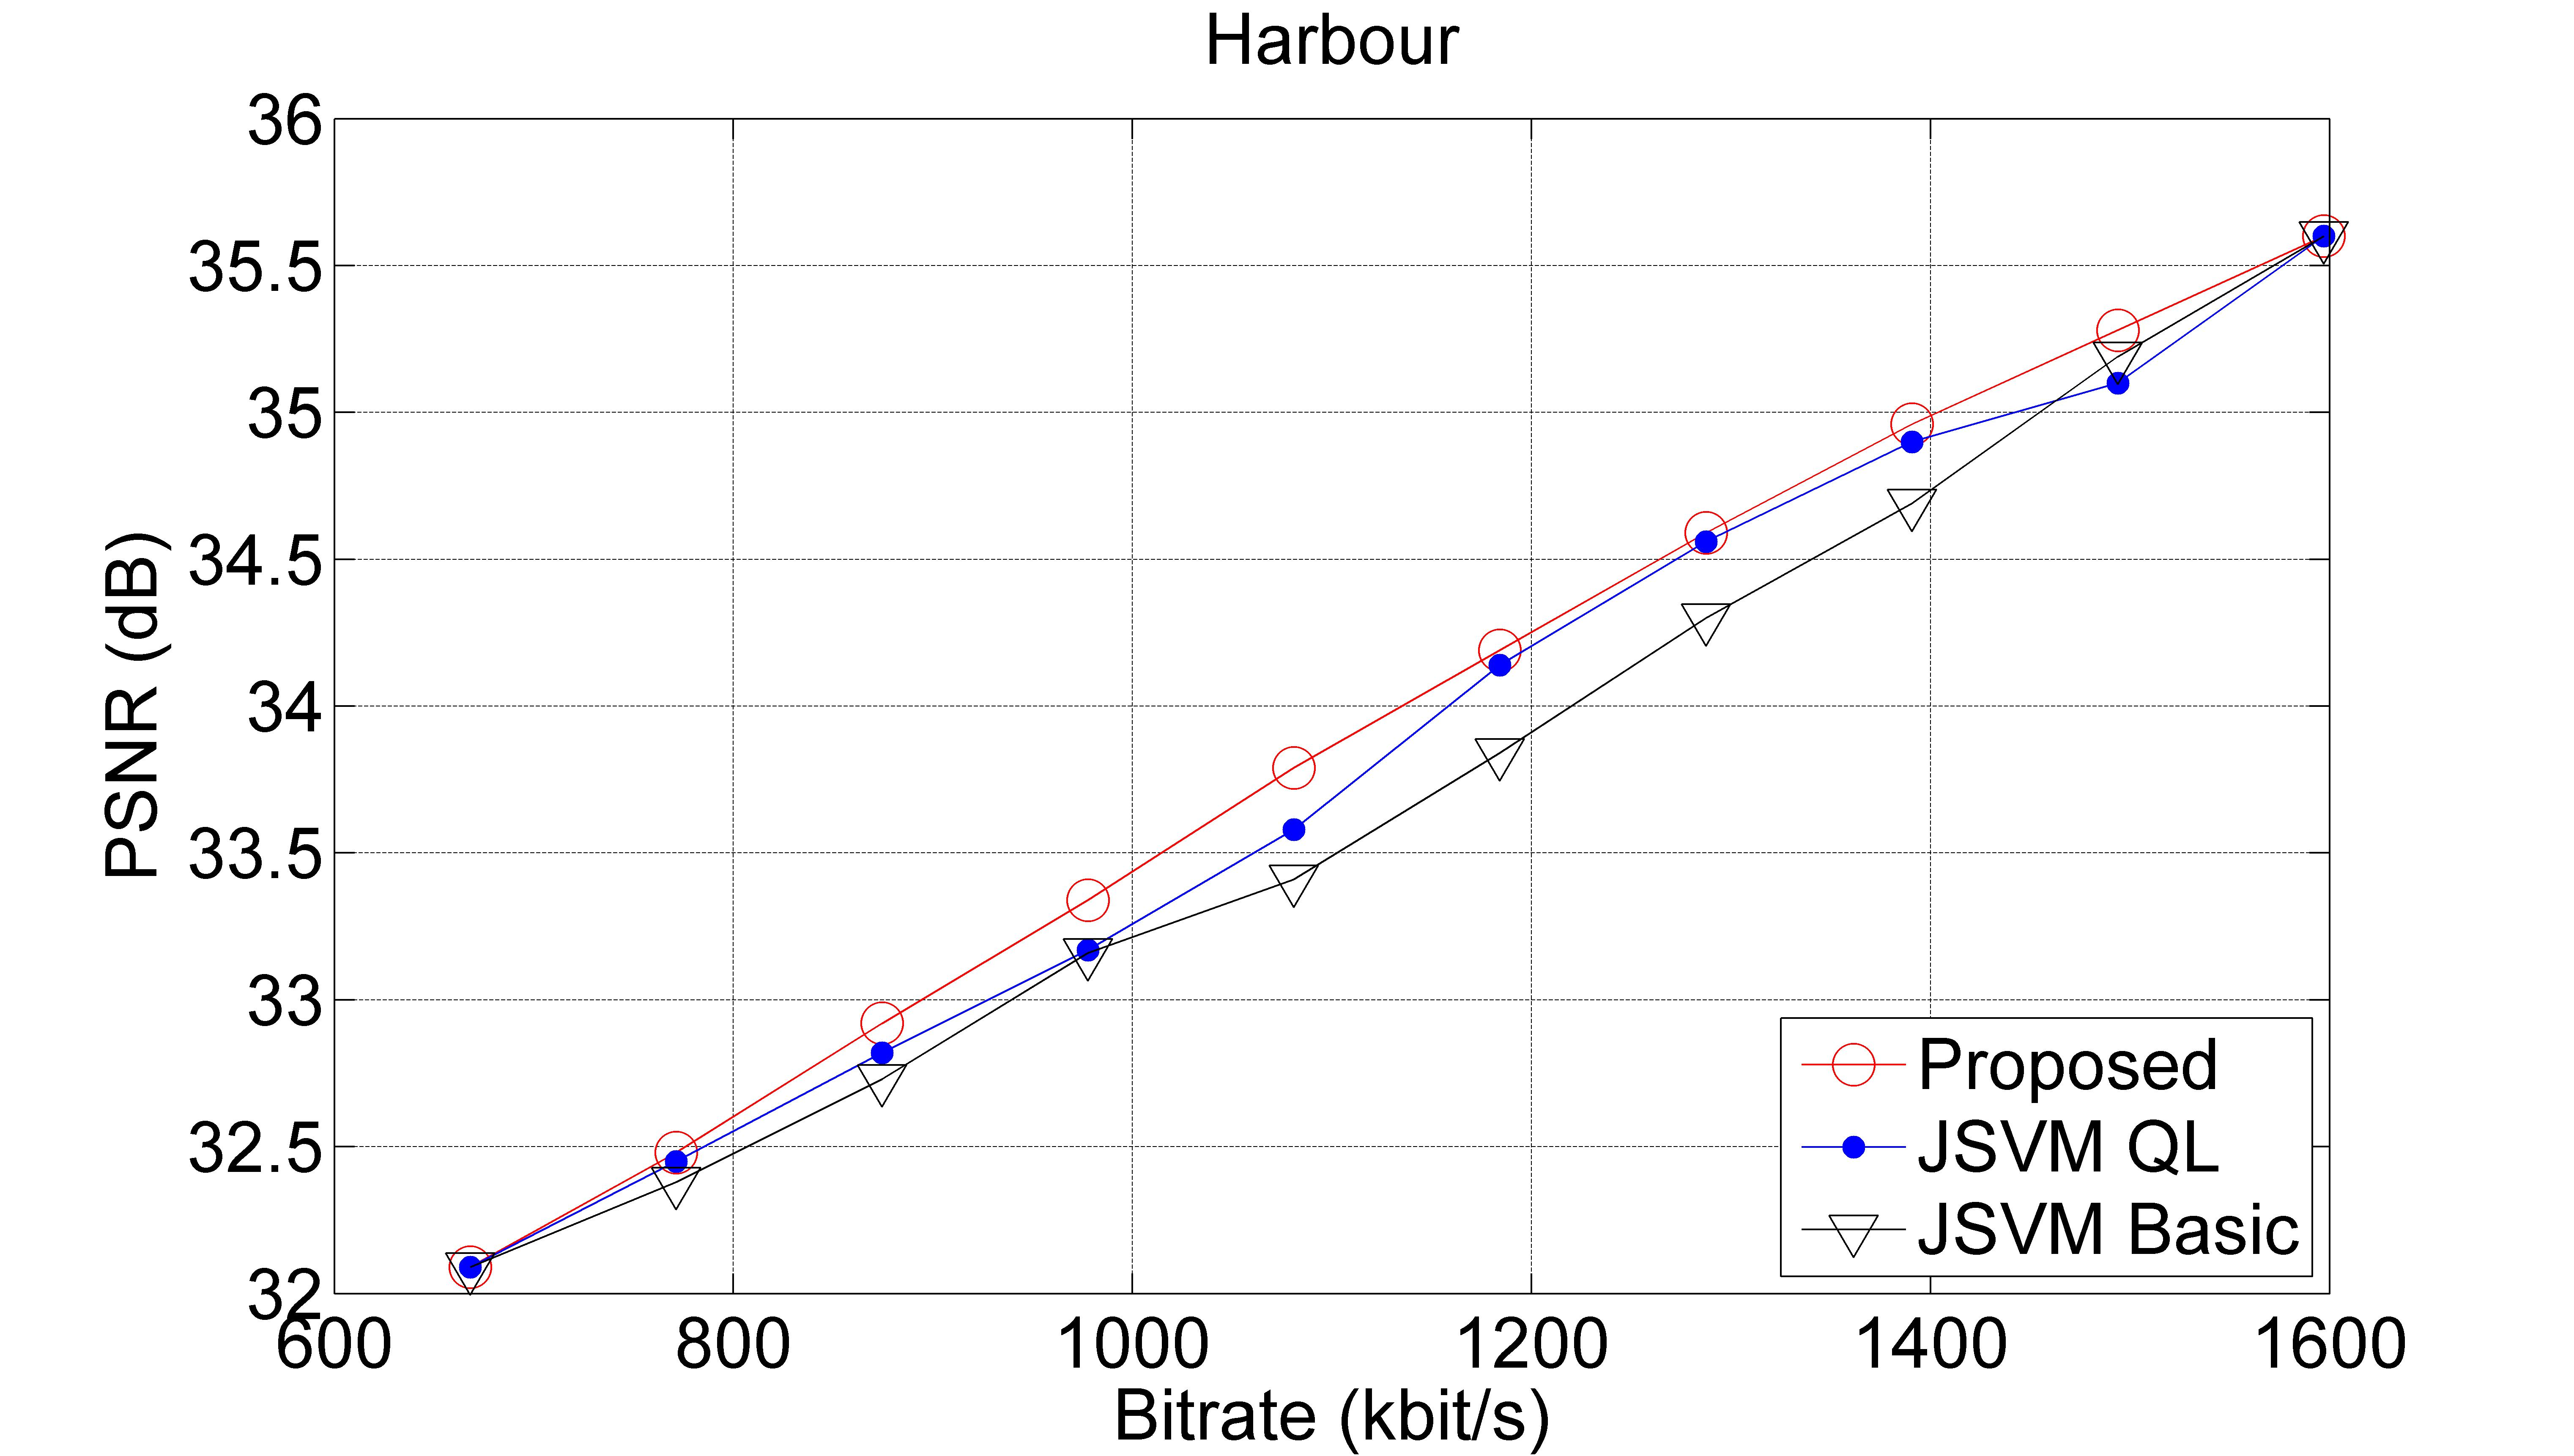
\includegraphics[width=0.5\textwidth]{Harbour.jpg}
\label{fig:Harbour}}
\subfloat[Soccer]{
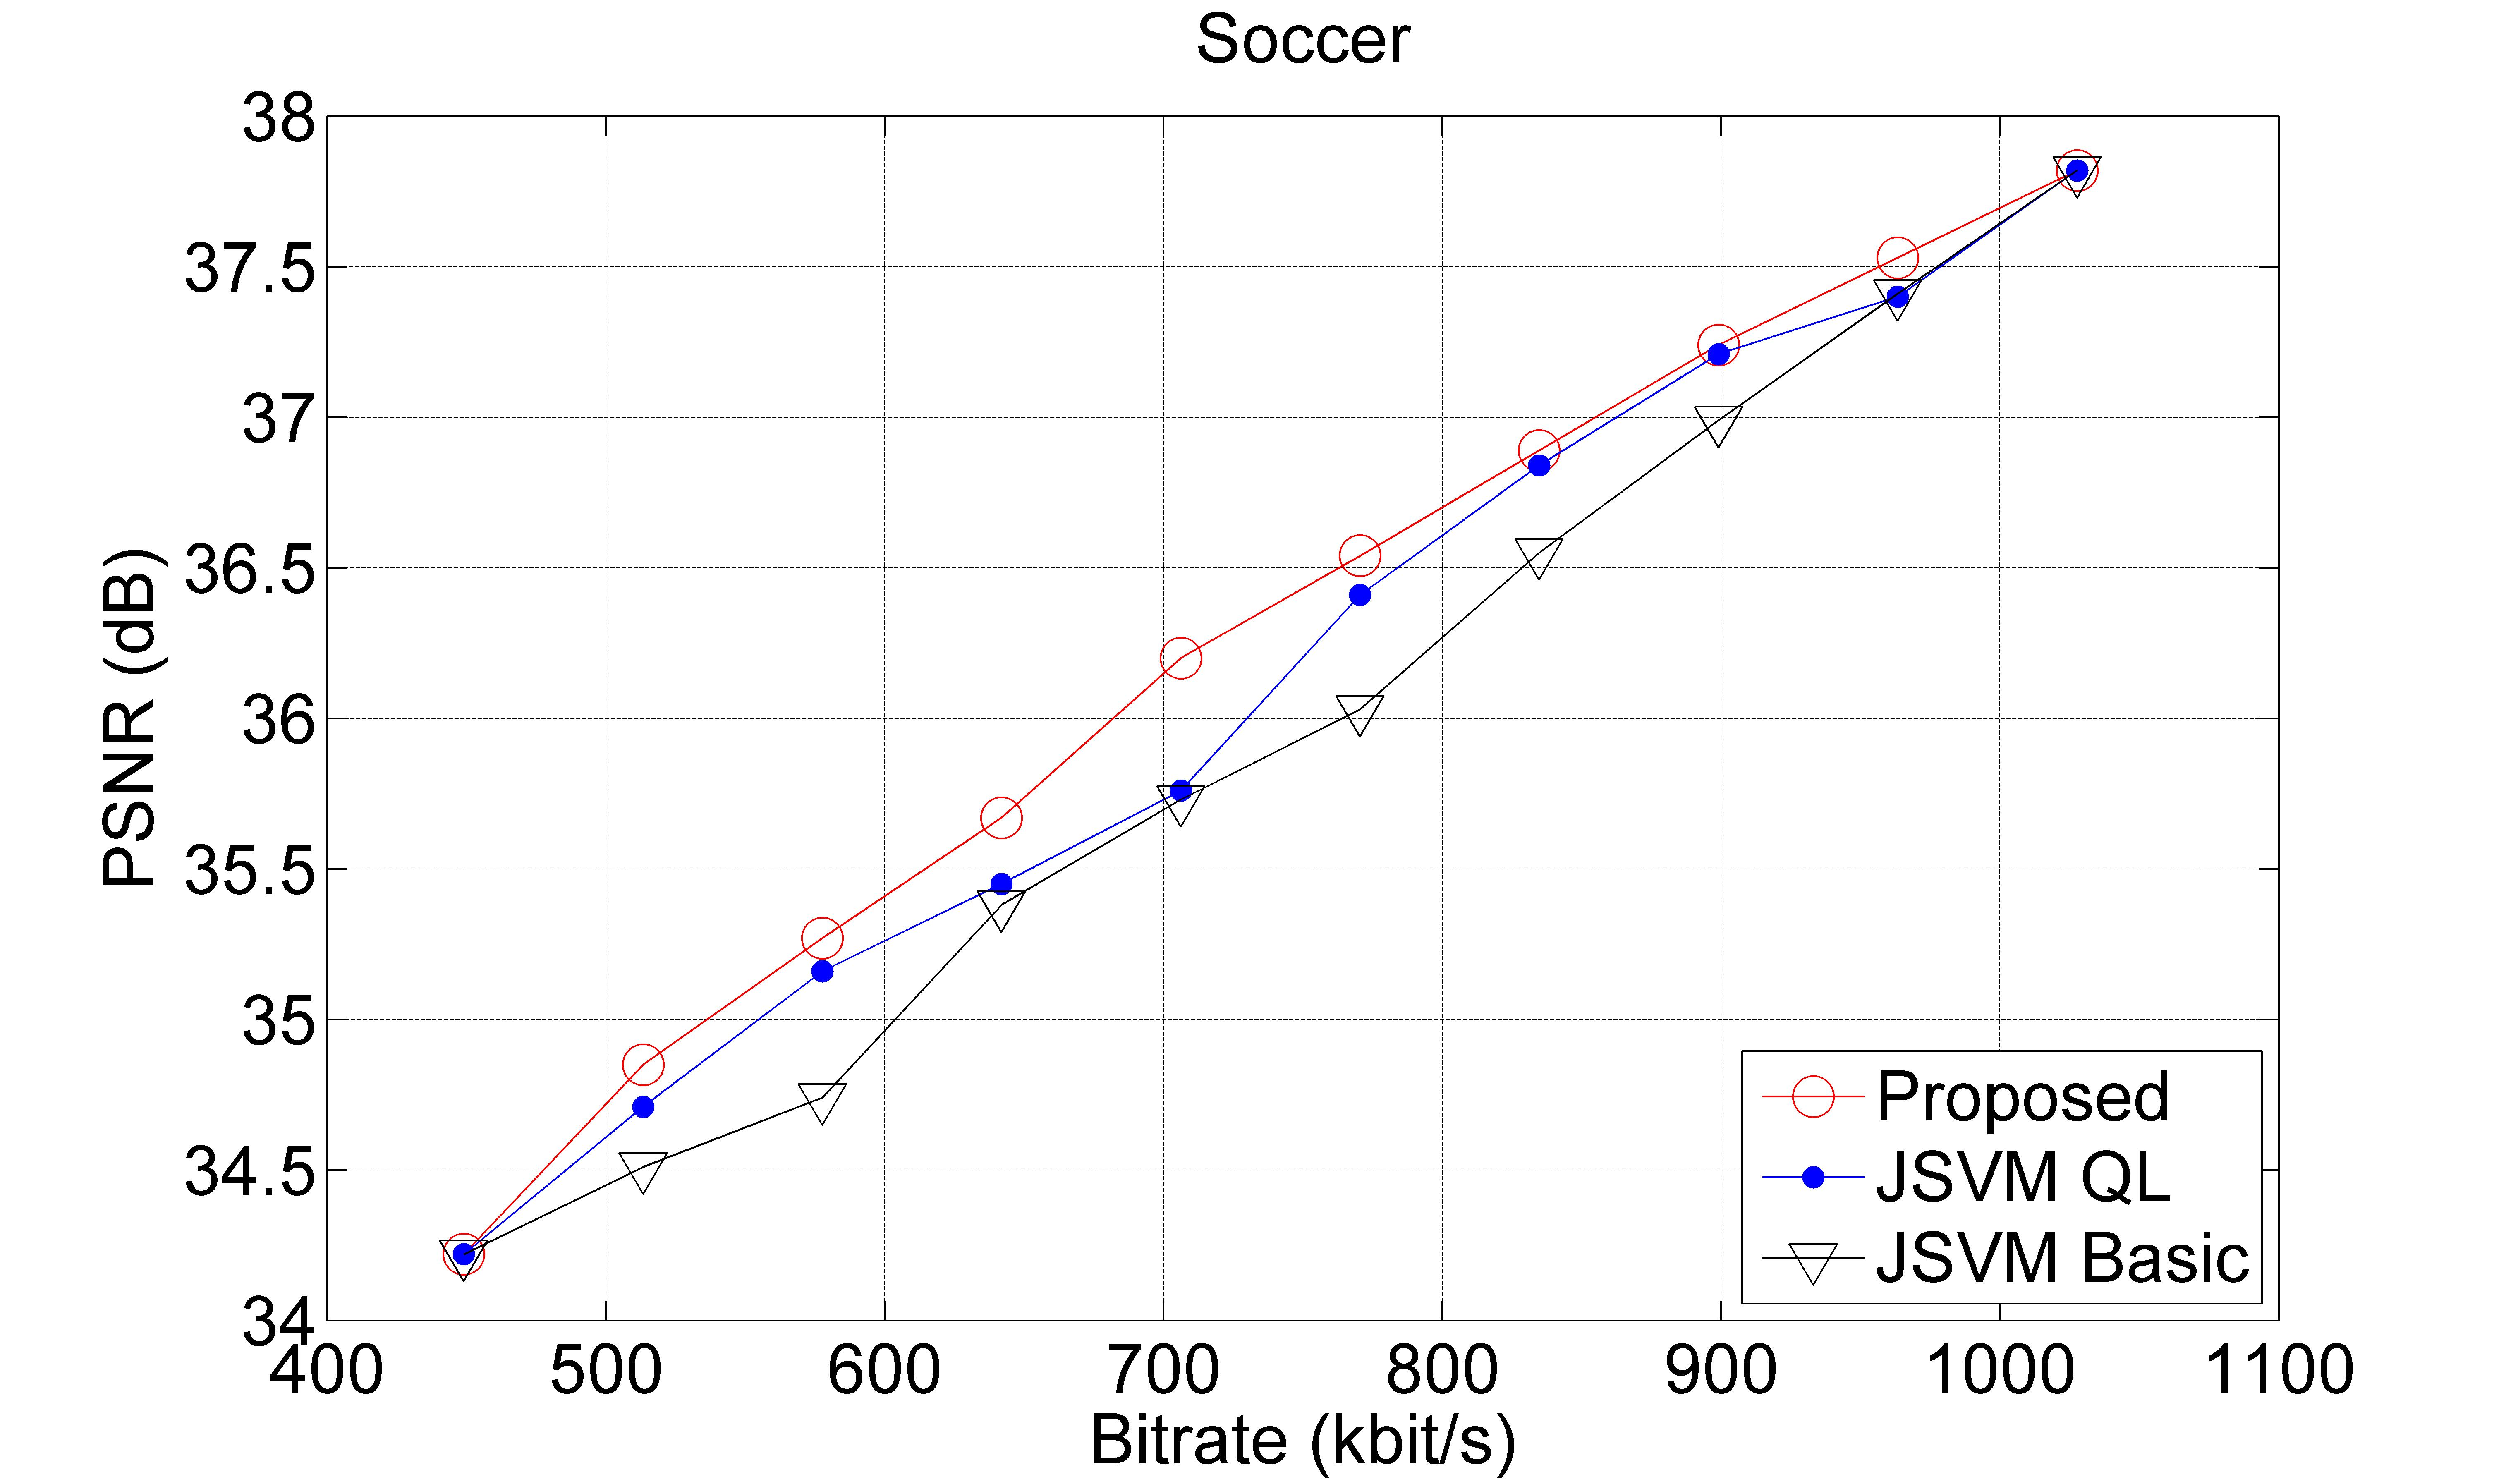
\includegraphics[width=0.5\textwidth]{Soccer.jpg}
\label{fig:Soccer}}
\caption{Performance of three bitstream extraction methods for various CIF sequences}
\label{fig:performance}
\end{figure*}

\begin{table*}[t]
\centering
\caption{Algorithm Performance: Luma PSNR Gain Compared with JSVM}
\label{tab:results}
\begin{minipage}{0.95\linewidth}
% \renewcommand{\thefootnote}{\thempfootnote}
\centering
\begin{tabular}{c|c|p{1.2cm}<{\centering}|p{1.2cm}<{\centering}|p{1.2cm}<{\centering}|p{1.2cm}<{\centering}| 
p{1.2cm}<{\centering}|p{1.2cm}<{\centering}|p{1.2cm}<{\centering}|p{1.2cm}<{\centering}}
%% |l|l| to left justify each column entry
%% |c|c| to center each column entry
%% use of \rule[]{}{} below opens up each row 
\hline \hline
\multicolumn{2}{c|}{Sequence} &
{\em Bus} & {\em City} & {\em Crew} & {\em Football} & {\em Foreman} & {\em Harbour} & {\em Mobile} & {\em Soccer} \\ \hline 
\multirow{2}{*}{JSVM QL\footnote{\label{footnote:JSVM_QL} Comparing the proposed algorithm with JSVM QL} (dB)}
& Max\footnote{\label{footnote:max} Maximum PSNR gain through all bitrate constraints} & 0.37 & 0.50 & 0.13 & 0.22 & 0.23 & 0.19 & 0.25 & 0.44 \\ \cline{2-10}
& Ave\footnote{\label{footnote:ave} Average PSNR gain through all bitrate constraints} & 0.11 & 0.11 & 0.05 & 0.12 & 0.05 & 0.05 & 0.06 & 0.13 \\ \hline
\multirow{2}{*}{JSVM no QL (dB)}
& Max & 0.50 & 0.83 & 0.32 & 0.29 & 0.50 & 0.34 & 0.61 & 0.53 \\ \cline{2-10}
& Ave & 0.18 & 0.37 & 0.20 & 0.15 & 0.22 & 0.15 & 0.25 & 0.29 \\ \hline
\end{tabular}
\end{minipage}
\end{table*}

\subsection{Experiments for Quality Control}
\label{subsec:exp-control}

For simplicity and intuition, we combine the enhancement layers in the tested SVC video stream to construct quality levels (introduced in \ref{subsec:quality-level}) used in the quality control algorithm. The video stream is divided into several sub-streams, each of which is identified by the quality and temporal layer it contains, as illustrated in Table \ref{tab:sub-stream} (there are 3 layers in each scalability dimension; spatial scalability is not enabled). The quality level is defined as the sum of all sub-streams with ID equal or less than the level number. For example, quality level 3 would contain all sub-streams from 0 to 3, thus would include all temporal layers, but only the quality base layer 0. The tested stream has 9 quality levels from 0 to 8 (see Table \ref{tab:sub-stream}), and a maximum bit rate of 1587 kbps at level 8. 

\begin{table*}[t]
\centering
\caption{Sub-stream ID}
\label{tab:sub-stream}
\begin{tabular}{c|*{8}{p{1.2cm}<{\centering}|}{p{1.2cm}<{\centering}}}
	\hline\hline
	  Sub-stream ID   & 0 & 1 & 2 & 3 & 4 & 5 & 6 & 7 & 8 \\ \hline
	Quality Layer ID  & 0 & 0 & 0 & 1 & 1 & 1 & 2 & 2 & 2 \\ \hline
	Temporal Layer ID & 0 & 1 & 2 & 0 & 1 & 2 & 0 & 1 & 2 \\ \hline
\end{tabular}
\end{table*}

We simulate network fluctuation by adjusting bandwidth around a certain level. We set this level from 400 to 1400 kbps to reflect different average bandwidth. All the experiments are conducted with DSS as the software platform, and the bandwidth simulation is implemented with NetLimiter 3 \cite{Netlimiter}. The baseline algorithm in the comparison refers to the packet delay feedback (PDF) algorithm in the original DSS.

First of all, we conduct some preliminary improvement experiments using only proportional part or integral part of the PID model. Since they are directly related to the short term error and long term error respectively, we call them Short Term Prediction (STP) and Long Term Prediction (LTP). Fig. \ref{fig:performance-all} shows the experimental results of these two control algorithms and the baseline algorithm. In the figures, the video quality is measured by the quality level defined in the beginning of this section, and quality smoothness is indicated by the variance of the quality levels along time. We can conclude that STP provides the best average quality level at the expense of high quality variance. This can be easily explained since this quality control strategy closely follows the bandwidth fluctuation. In contrast, LTP keeps a relatively low quality variance at a little cost of average video quality. Although it is not as good as STP in average quality, it still outperforms the baseline algorithm by 7.9\%.

Since STP and LTP have their own limitations, we implement the complete PID-based quality control algorithm, which can both reduce quality variance and improve average quality level. From the result shown in Fig. \ref{fig:performance-two}, we can conclude that when integrated with integral part and derivative part, the effect of proportional part is not as aggressive as in STP. An obvious proof can be found in Fig. \ref{fig:variance-two}, which clearly shows that the proposed PID quality control algorithm keeps a lower quality variance compared to PDF algorithm. Table \ref{tab:improvement} lists the statistical experimental results for these four quality control algorithms, in which PID-based control algorithm has shown its advantage over the others, especially in reducing the quality fluctuation. It can be seen that, compared to PDF, the PID-based quality control algorithm improves 8.6\% in video quality with 24.8\% reduction in quality fluctuation. The video quality fluctuation of the four control algorithms, when available bandwidth fluctuates around 800 kbps, is shown in Fig. \ref{fig:fluctuation}, from which we can see a more stable video quality in the proposed PID quality control algorithm.

\begin{figure*}[t]
\subfloat[Average quality level of different control algorithms]{
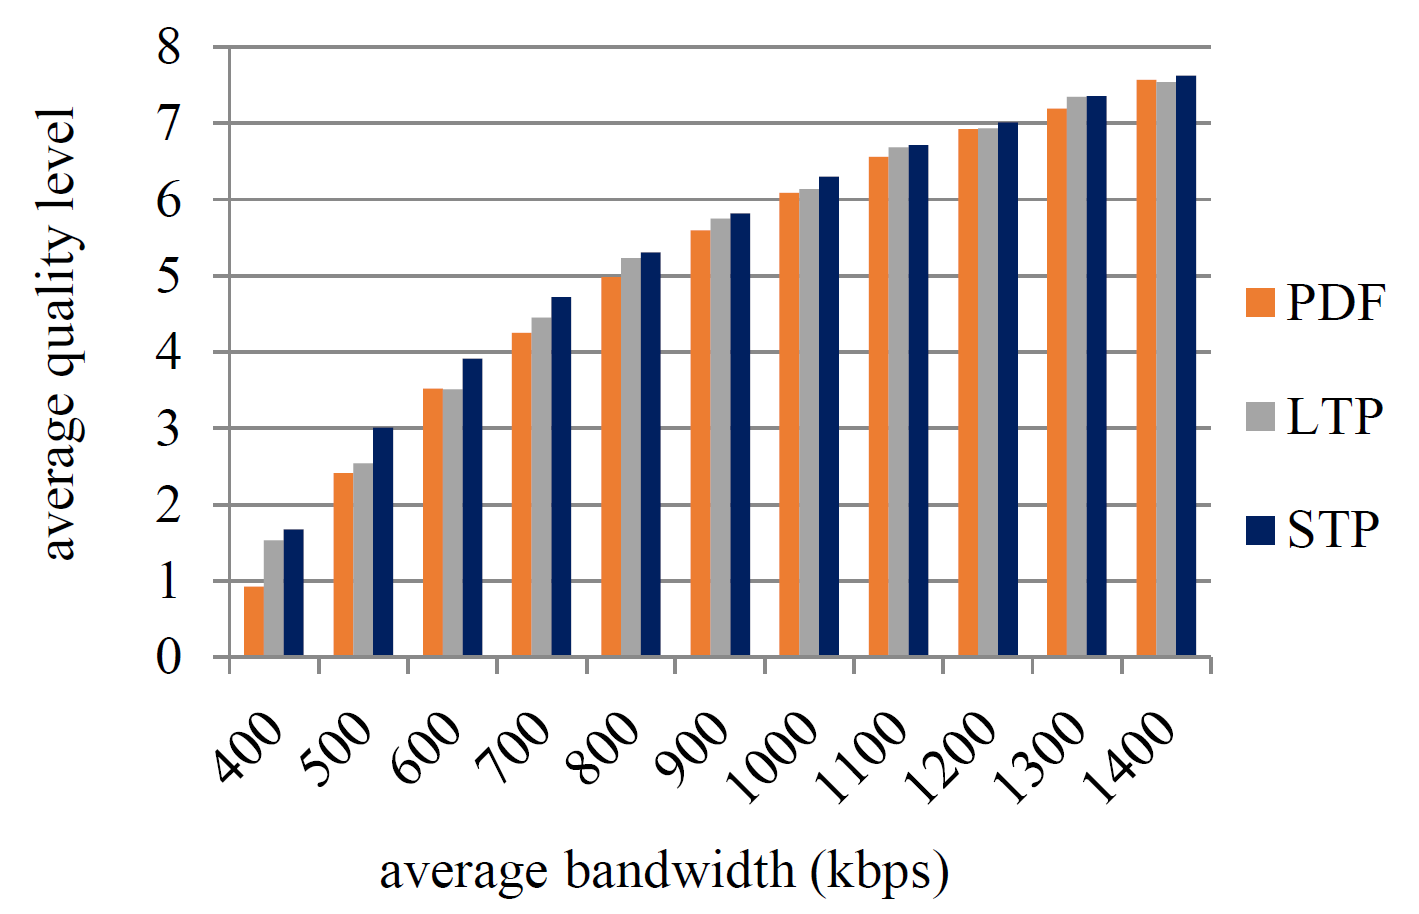
\includegraphics[width=0.5\textwidth]{Quality-all.png}
\label{fig:quality-all}}
\subfloat[Variance of quality level of different control algorithms]{
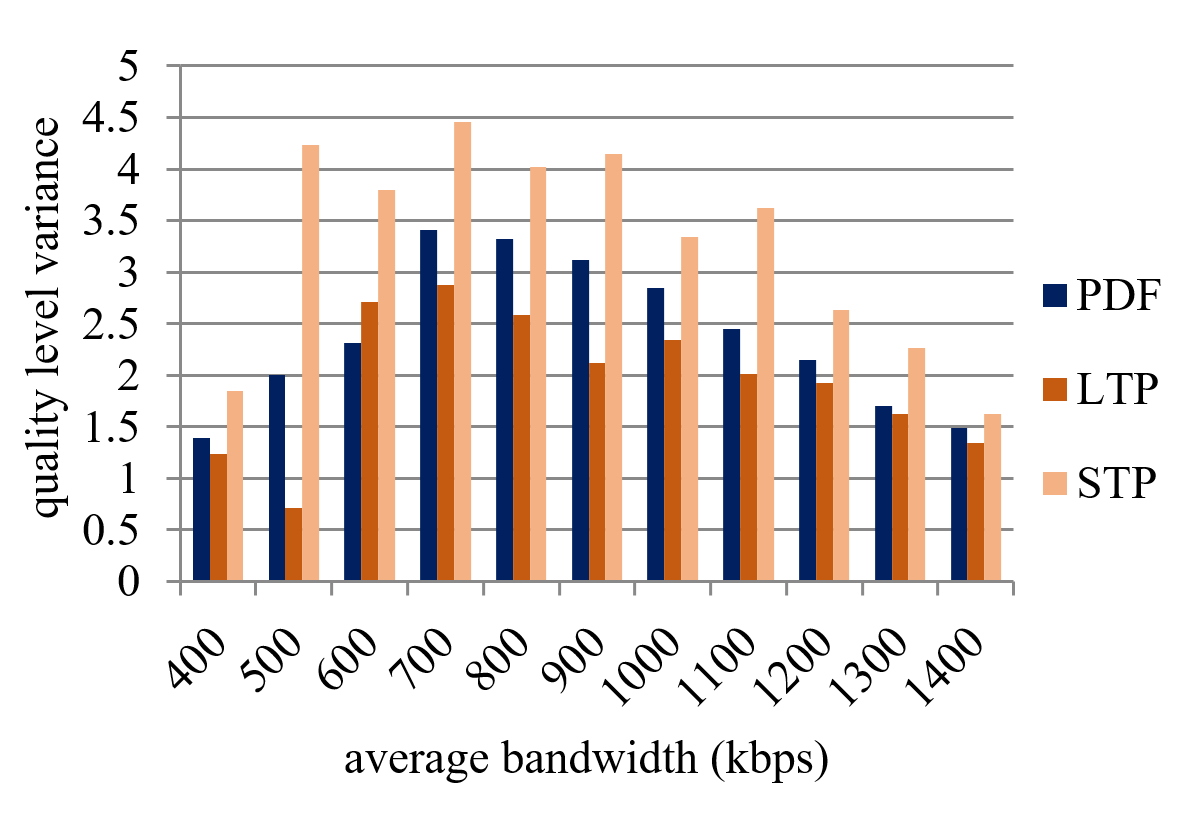
\includegraphics[width=0.5\textwidth]{Variance-all.png}
\label{fig:variance-all}}
\caption{Comparison of the long/short time prediction and the PDF algorithm in DSS}
\label{fig:performance-all}
\end{figure*}

\begin{figure*}[t]
\centering
\subfloat[Variance of quality level of PID and PDF control algorithms]{
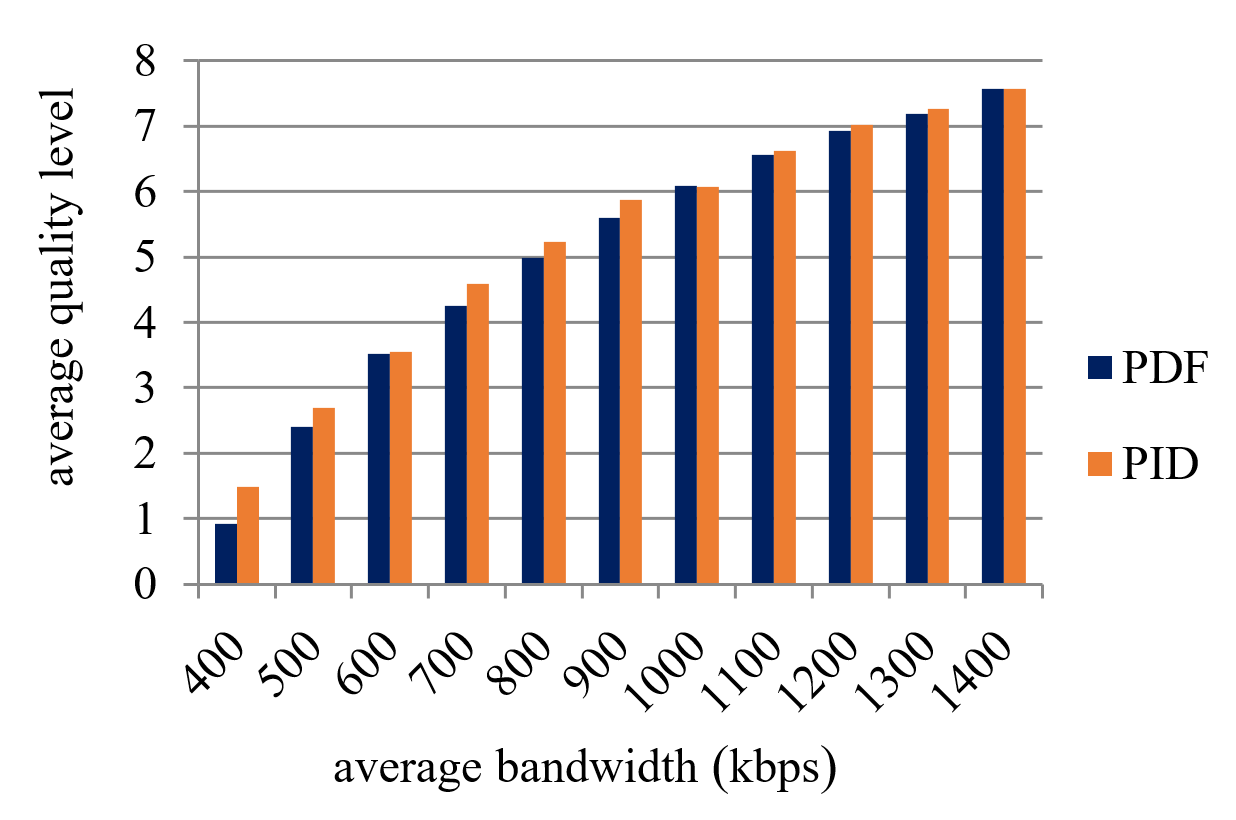
\includegraphics[width=0.5\textwidth]{Quality-two.png}
\label{fig:quality-two}}
\subfloat[Average quality level of PID and PDF control algorithms]{
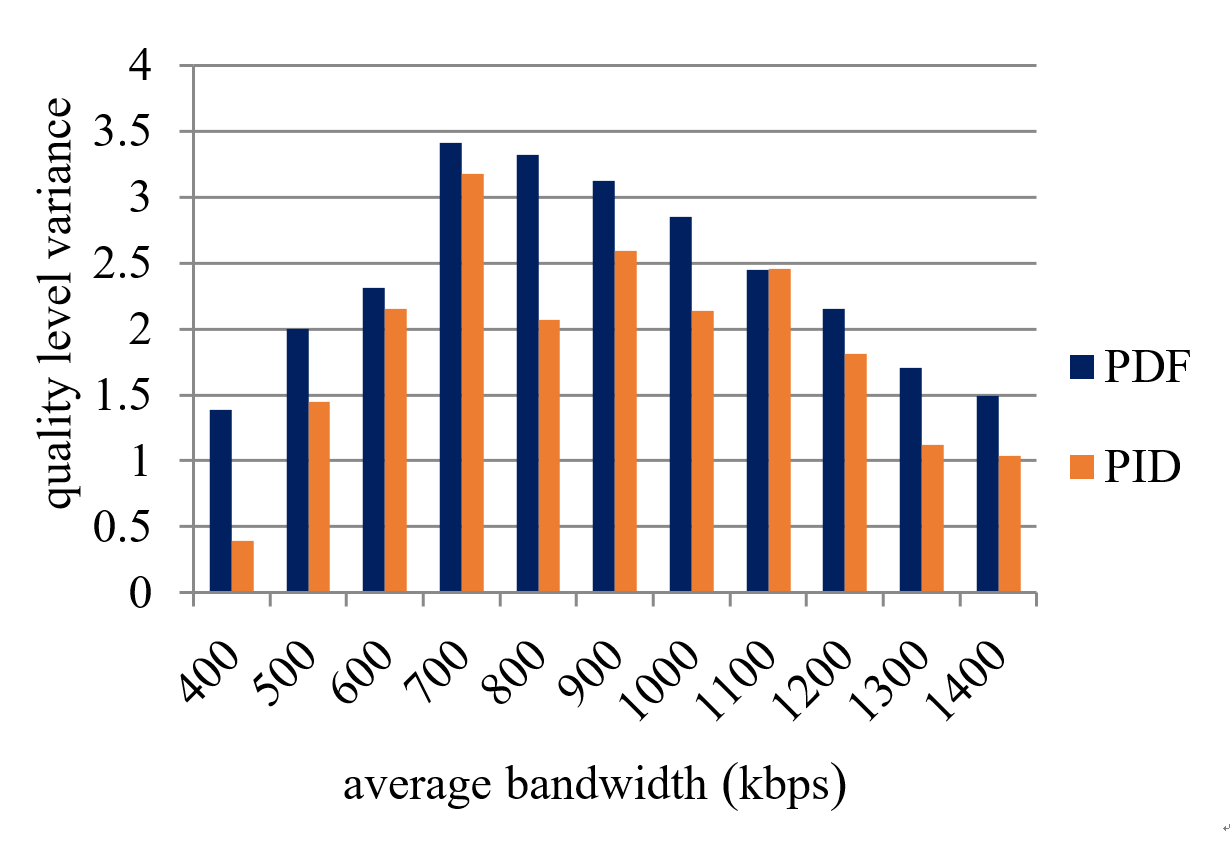
\includegraphics[width=0.5\textwidth]{Variance-two.png}
\label{fig:variance-two}}
\caption{Comparison of the proposed PID algorithm and the PDF algorithm in DDS}
\label{fig:performance-two}
\end{figure*}


\begin{table*}[t]
\centering
\caption{Improvement of Different Quality Control Schemes}
\label{tab:improvement}
\begin{tabular}[b]{p{4.2cm}<{\centering}|p{4.2cm}<{\centering}|p{4.2cm}<{\centering}}
\hline \hline
Quality control scheme & Average quality level & Quality variance \\ \hline
Packet delay feedback (PDF) & 0.0\% & 0.0\% \\ \hline
Short term prediction (STP) & \textbf{+13.5\%} & +38.5\% \\ \hline
Long term prediction (LTP) & +7.9\% & -17.2\% \\ \hline
PID based control scheme(PID) & +8.6\% & \textbf{-24.8\%} \\ \hline
\end{tabular}
\end{table*}


\begin{figure}
\centering
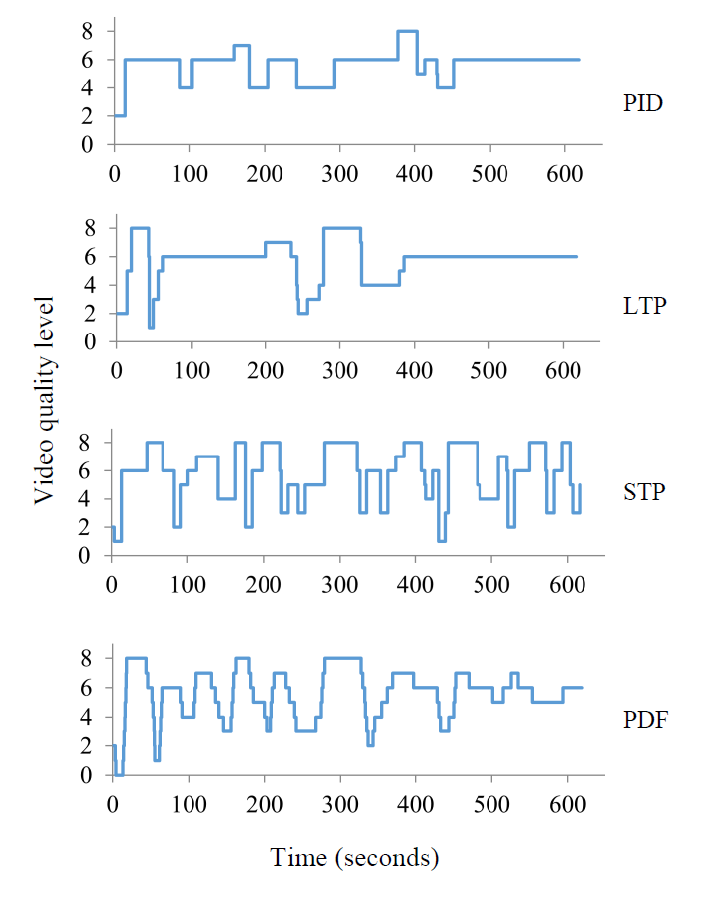
\includegraphics[width = 0.9\linewidth]{Fluctuation.png}
\caption{Video quality fluctuation with time \label{fig:fluctuation}}
\end{figure}

\subsection{Result of the Combined System}

After combining the two algorithms together, the proposed adaptive streaming system is able to deliver a higher and smoother video quality for the user. We compare the proposed system's performance with DSS that supports SVC but has its original quality control method and JSVM Basic bitstream extraction. The result for the same test stream as used in subsection \ref{subsec:exp-control} is present in Fig. \ref{fig:fluctuation-psnr}. It shows PSNR change perceived by the user when available bandwidth fluctuates around certain values (600kbps, 800kbps, 1000kbps and 1200kbps). The bandwidth conditions are simulated with NetLimiter and intense fluctuations are observed. It can be seen that, the proposed system performs better in that it has effectively avoided unnecessary quality drop (e.g., note the curve around time 450s in Fig. \ref{fig:Fluctuation-PSNR1} or 250s in Fig. \ref{fig:Fluctuation-PSNR3}) and been able to keep a relatively higher PSNR value (e.g., note the curve around time 400s in Fig. \ref{fig:Fluctuation-PSNR2} or 500s in Fig. \ref{fig:Fluctuation-PSNR4}). The average and variance value of PSNR is also calculated and present in Fig. \ref{fig:fluctuation-psnr}, showing clearly the proposed system's advantage. For instance, in Fig. \ref{fig:Fluctuation-PSNR4} where bandwidth fluctuates around 1200kbps, the average PSNR delivered by the proposed system is 41.14dB, 0.66dB higher than that of the baseline system, and the PSNR variance is also reduced from 0.63 to 0.21, indicating a more smooth video quality change.


\begin{figure*}[t]
\centering
\subfloat[Bandwidth fluctuates around 600kbps: PSNR average and variance in the original system are 39.63 and 0.24, while in the proposed system are 39.69 (increased by 0.06) and 0.16 (reduced by 0.08).]{
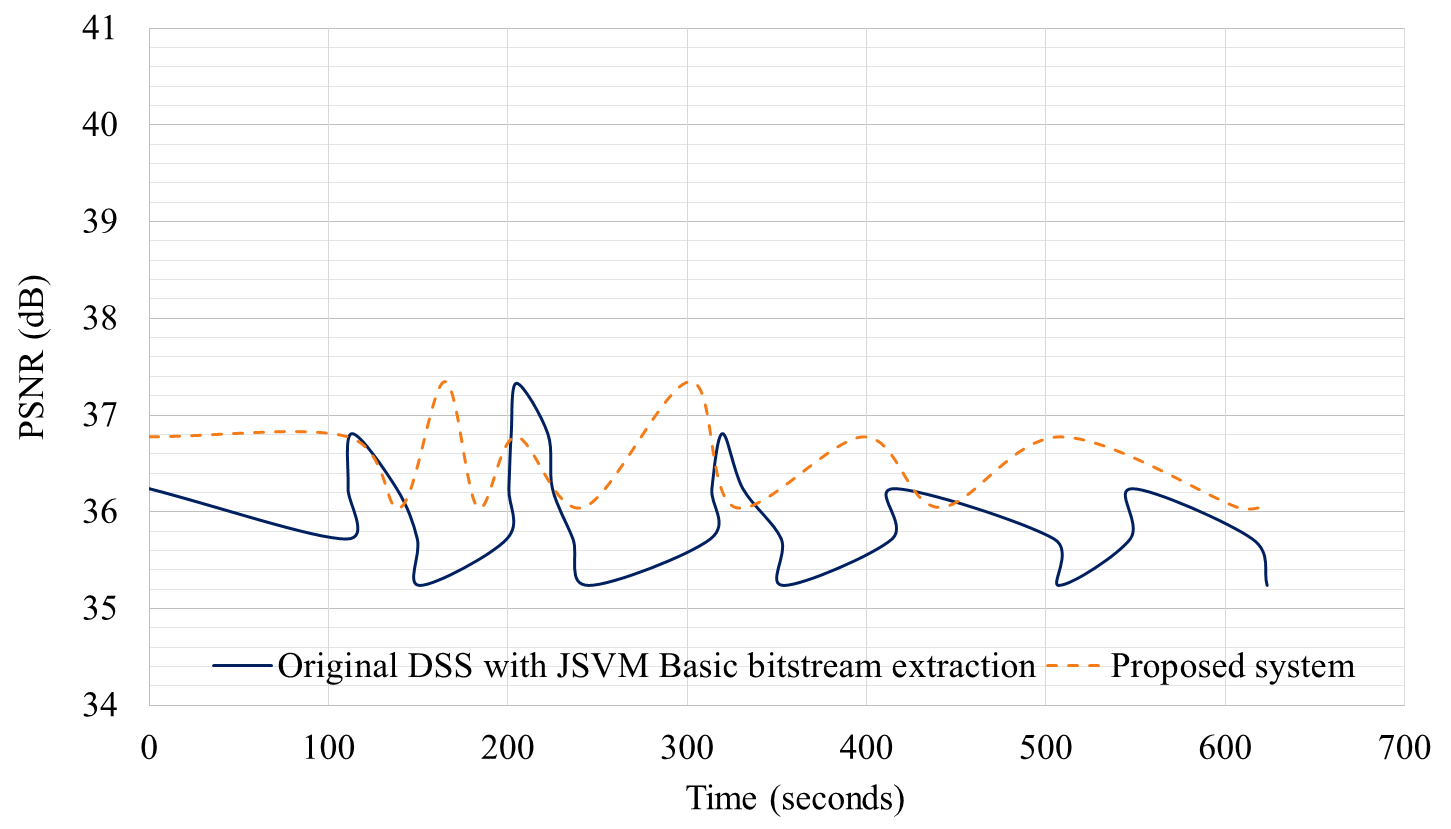
\includegraphics[width=0.47\textwidth]{Fluctuation-PSNR1.png}
\label{fig:Fluctuation-PSNR1}}\hfill
\subfloat[Bandwidth fluctuates around 800kbps: PSNR average and variance in the original system are 40.15 and 0.48, while in the proposed system are 40.62 (increased by 0.47) and 0.28 (reduced by 0.20).]{
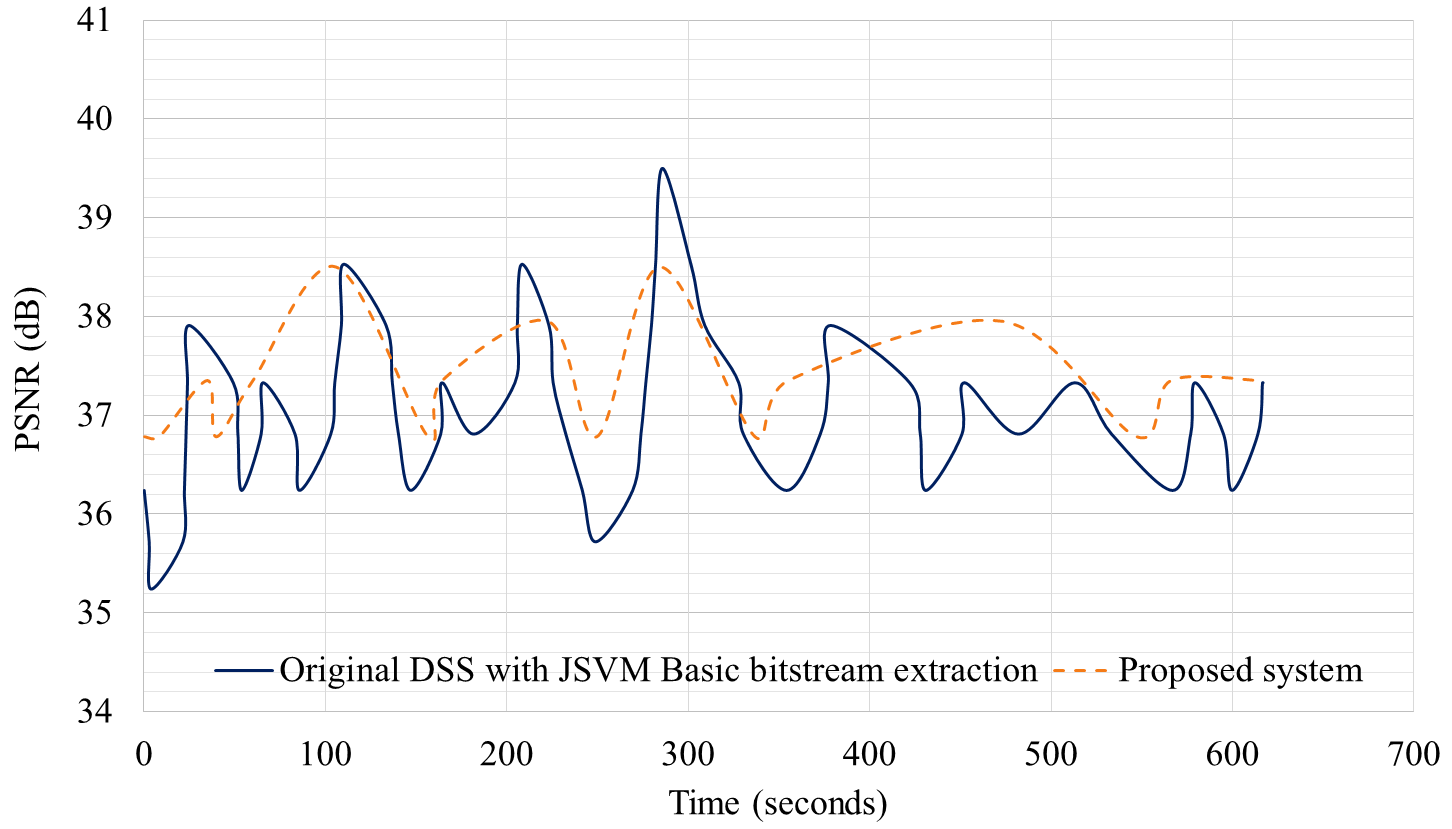
\includegraphics[width=0.47\textwidth]{Fluctuation-PSNR2.png}
\label{fig:Fluctuation-PSNR2}}
\qquad
\subfloat[Bandwidth fluctuates around 1000kbps: PSNR average and variance in the original system are 40.37 and 0.50, while in the proposed system are 40.74 (increased by 0.40) and 0.28 (reduced by 0.22).]{
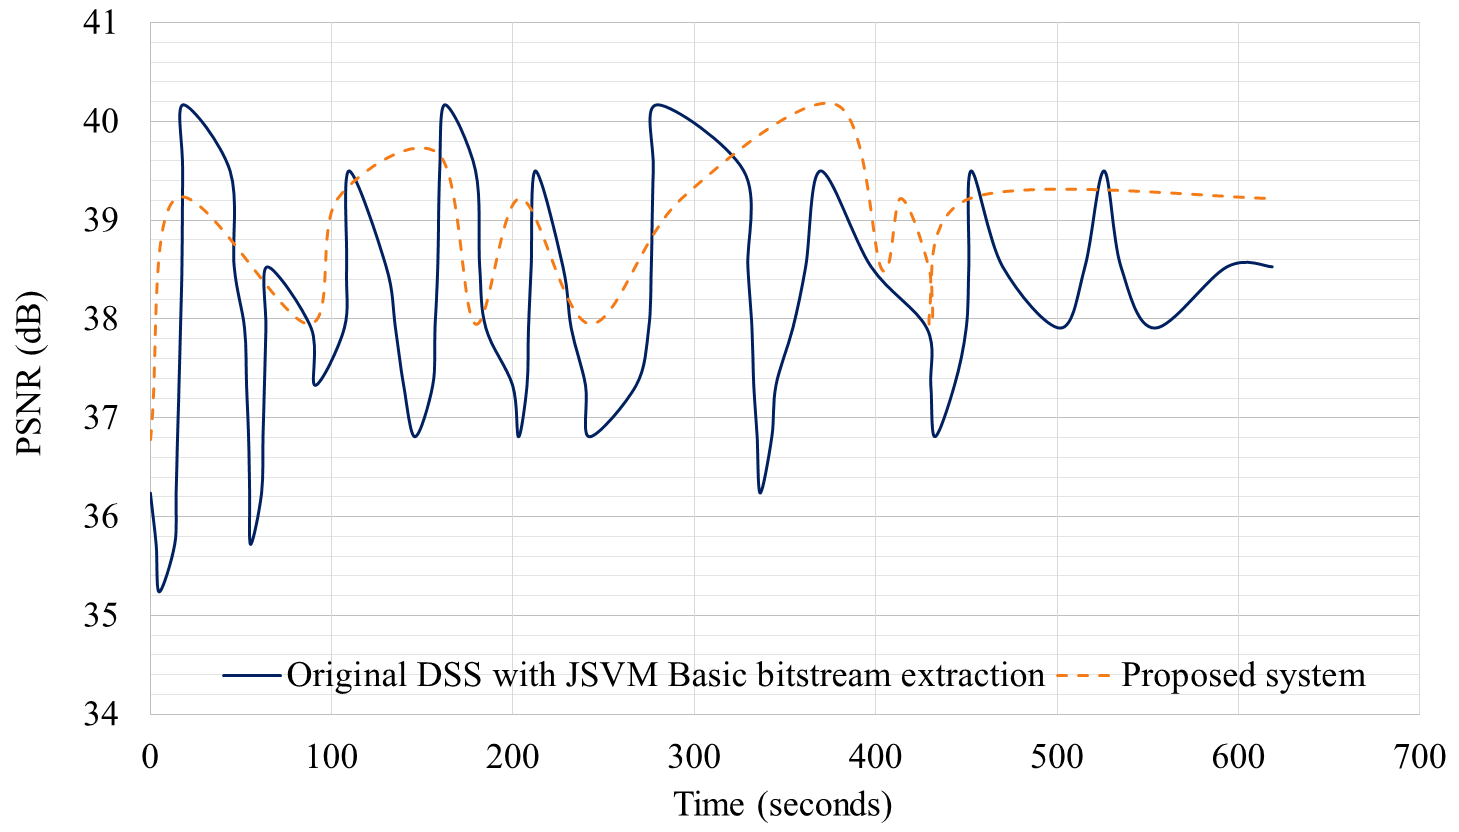
\includegraphics[width=0.47\textwidth]{Fluctuation-PSNR3.png}
\label{fig:Fluctuation-PSNR3}}\hfill
\subfloat[Bandwidth fluctuates around 1200kbps: PSNR average and variance in the original system are 40.48 and 0.63, while in the proposed system are 41.14 (increased by 0.66) and 0.21(reduced by 0.42).]{
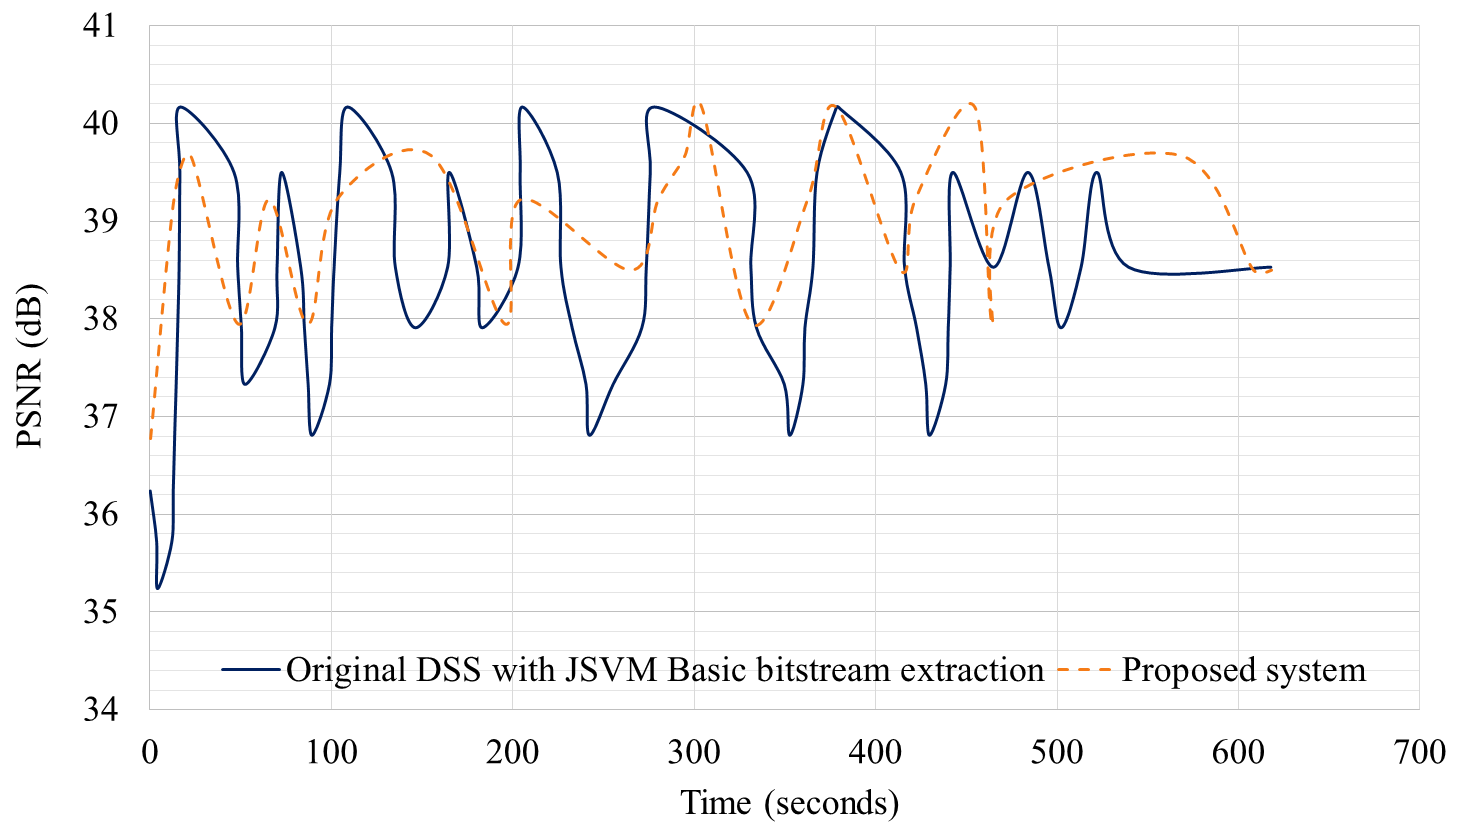
\includegraphics[width=0.47\textwidth]{Fluctuation-PSNR4.png}
\label{fig:Fluctuation-PSNR4}}
\caption{User-perceived PSNR change with time when bandwidth fluctuates \label{fig:fluctuation-psnr}}
\end{figure*}

\section{Conclusion}
\label{sec:conclusion}

In this paper, an adaptive video streaming system with optimized bitstream extraction and PID-based quality control is proposed. The bitstream extraction method includes a linear error model to estimate the distortion caused by discarding any combination of packets and a greedy algorithm to assign priority to each data packet. The priority values can then be stored in the bitstream and used for R-D optimized extraction. Experimental results show that the method can achieve PSNR gain of up to 0.5dB compared to the JSVM QL extractor under the same bitrate constraint, also with the same computational complexity. The PID-based quality control algorithm has a flexible mechanism to determine the suitable quality level so that it gives an accurate and swift response to the bandwidth change. Comparing with the original algorithm in DSS, this algorithm has reduced quality fluctuation significantly to improve audience satisfaction. The proposed SVC adaptive streaming system integrated with these two solutions performs well in automatically adapting to the user's bandwidth fluctuation, and is able to give the user a better watching experience.

Since the next generation video coding standard High Efficiency Video Coding (HEVC) \cite{HEVC} adopts the similar coding framework as its predecessor H.264/AVC, we expect to apply this paper's model and approach of bitstream extraction to the emerging HEVC standard and its scalable extension. As for the PID-based quality control algorithm, it is only network-concerned thus should be easily integrated into other streaming systems, e.g., simulcast system like DASH.


% Can use something like this to put references on a page
% by themselves when using endfloat and the captionsoff option.
\ifCLASSOPTIONcaptionsoff
  \newpage
\fi



% trigger a \newpage just before the given reference
% number - used to balance the columns on the last page
% adjust value as needed - may need to be readjusted if
% the document is modified later
%\IEEEtriggeratref{8}
% The "triggered" command can be changed if desired:
%\IEEEtriggercmd{\enlargethispage{-5in}}

% references section

% can use a bibliography generated by BibTeX as a .bbl file
% BibTeX documentation can be easily obtained at:
% http://www.ctan.org/tex-archive/biblio/bibtex/contrib/doc/
% The IEEEtran BibTeX style support page is at:
% http://www.michaelshell.org/tex/ieeetran/bibtex/
%\bibliographystyle{IEEEtran}
% argument is your BibTeX string definitions and bibliography database(s)
%\bibliography{IEEEabrv,../bib/paper}
%
% <OR> manually copy in the resultant .bbl file
% set second argument of \begin to the number of references
% (used to reserve space for the reference number labels box)
\begin{thebibliography}{1}

\bibitem{Gualdi08}
G. Gualdi, A. Prati, and R. Cucchiara, ``Video Streaming for Mobile Video Surveillance'', in {\em IEEE Transactions on Multimedia}, vol. 10, no. 6, pp. 1142-1154, 2008.

\bibitem{Chen13}
Y. Chen, B. Zhang, Y. Liu, and W. Zhu, ``Measurement and Modeling of Video Watching Time in a Large-Scale Internet Video-on-Demand System'', in {\em IEEE Transactions on Multimedia}, vol. 15, no. 8, pp. 2087-2098, 2013.

\bibitem{Egilmez14}
H. E. Egilmez and A. M. Tekalp, ``Distributed QoS architectures for multimedia streaming over software defined networks'', in {\em IEEE Transactions on Multimedia}, vol. 16, no. 6, pp. 1597-1609, 2014.

\bibitem{Li14}
S. Li et al., ``Flexible Traffic Engineering (F-TE): When OpenFlow Meets Multi-Protocol IP-Forwarding'', in {\em IEEE Communication Letters}, vol. 18, pp. 1699-1702, Oct. 2014.

\bibitem{Xue15}
N. Xue et al., ``Demonstration of OpenFlow-Controlled Network Orchestration for Adaptive SVC Video Manycast'', in {\em IEEE Transactions on Multimedia}, vol. 17, pp. 1617-1629, Sept. 2015.

\bibitem{DASH}
T. Stockhammer, ``Dynamic adaptive streaming over HTTP: standards and design principles", in {\em Proceedings of the second annual ACM conference on Multimedia systems}, 2011.

\bibitem{SVC}
T.~Wiegand, G.~Sullivan, J.~Reichel, H.~Schwarz, M.~Wien, eds., ``Joint Draft ITU-T Rec. H.264|ISO/IEC 14496-10/Amd.3 Scalable Video Coding'', Joint Video Team, Doc. JVT-X201 Jul. 2007.

\bibitem{SVCOverview}
H.~Schwarz, D.~Marpe, and T.~Wiegand, ``Overview of the scalable video coding extension of the H.264/AVC standard'', in {\em IEEE Trans. Circuits. Syst. Video Technol.}, vol. 17, no. 9, pp. 1103-1120, 2007.

\bibitem{Bouten14}
N. Bouten, S. Latre, J. Famaey, W. V. Leekwijck, and F. D. Turck, ``In-Network Quality Optimization for Adaptive Video Streaming Services'', in {\em IEEE Transactions on Multimedia}, vol. 16, no. 8, pp. 2281-2293, 2014.

\bibitem{YouTube}
https://www.youtube.com/

\bibitem{SVCPerformance}
M. Wien , H. Schwarz and T. Oelbaum,  ``Performance Analysis of SVC'',  in {\em IEEE Trans. Circuits Syst. Video Technol.}, vol. 17, no. 9, pp. 1194-1203, 2007.

\bibitem{Chuah12}
S. Chuah, Z. Chen, and Y. Tan, ``Energy-Efficient Resource Allocation and Scheduling for Multicast of Scalable Video Over Wireless Networks'', in {\em IEEE Transactions on Multimedia}, vol. 14, no. 4, pp. 1324-1336, 2012.

\bibitem{Zhu13}
Z. Zhu, S. Li, and X. Chen, ``Design QoS-aware multi-path provisioning strategies for efficient cloud-assisted SVC video streaming to heterogeneous clients'', in {\em IEEE Transactions on Multimedia}, vol. 15, no. 4, pp. 758-768, 2013.

\bibitem{Dan13}
G. Dan, O. Hadar, R. Ohayon, and N. Amram, ``Live video streaming with adaptive pre-processing by using scalable video coding'', in {\em Proceedings of IEEE International Conference on Consumer Electronics (ICCE)}, pp. 588-589, 2013.

\bibitem{Yang14}
E. Yang, Y. Ran, S. Chen, and J. Yang, ``A multicast architecture of SVC streaming over OpenFlow networks'', in {\em Proceedings of IEEE Global Communications Conference (GLOBECOM)}, pp. 1323-1328, 2014.

\bibitem{Cicalo14}
S. Cicalo, and V. Tralli, ``Distortion-Fair Cross-Layer Resource Allocation for Scalable Video Transmission in OFDMA Wireless Networks'', in {\em IEEE Transactions on Multimedia}, vol. 16, no. 3, pp. 848-863, 2014.

\bibitem{DSS}
http://dss.macosforge.org/

\bibitem{Knapsack}
http://en.wikipedia.org/wiki/Knapsack\_problem

\bibitem{Amonou07}
I.~Amonou, N.~Cammas, S.~Kervadec, S.~Pateux, ``Optimized Rate-distortion Extraction with Quality Layers in the Scalable Extension of H.264/AVC'' in {\em IEEE Trans. Circuits Syst. Video Technol.}, vol. 17, no. 9, pp. 1186-1193, 2007.

\bibitem{JSVM}
Text of ISO/IEC 14496-4:2001/PDAM 19 Reference Software for SVC, Joint Video Team (JVT) of ISO-IEC MPEG \& ITU-T VCEG, N9195, Sep. 2007.

\bibitem{Sun09}
J.~Sun, W.~Gao, D.~Zhao, W.~Li, ``On Rate-distortion Modeling and Extraction of H.264/SVC Fine-Granular Scalable Video'' in {\em IEEE Trans. Circuits Syst. Video Technol.}, vol.~19, no.~3, pp.~323-336, Mar. 2009.

\bibitem{Maani09}
E.~Maani, A.~K. Katsaggelos, ``Optimized Bit Extraction Using Distortion Modeling in the Scalable Extension of H.264/AVC'' in {\em IEEE Trans. Image Processing}, vol.~18, no.~9, pp.~2022-2029, 2009.

\bibitem{Ramanathan12}
P.~Ramanathan and N.~Jayant. ``RD optimized bitstream extraction for H. 264/SVC based video streaming'' In {\em Proceedings of IEEE International Conference on Image Processing}, pp. 2241-2244, 2012.

\bibitem{Yang13}
K.~Yang, S.~Wan, Y.~Gong, and Y.~Feng. ``A fast algorithm of bitstream extraction using distortion prediction based on simulated annealing'' In {\em Journal of Visual Communication and Image Representation}, no.7, pp. 752-759, 2013.

\bibitem{Zhang12}
W.~Zhang, J.~Sun, J.~Liu and Z.~Guo, ``Optimized bit extraction of SVC exploiting linear error model,'' {\em Proceedings of IEEE International Symposium on Circuits and Systems}, pp.~1887-1890, Seoul, Korea, May 2012.

\bibitem{Gao06}
K. Gao, J. Zhai, J. Li and C. Wang, ``Real-Time scheduling for scalable video coding streaming system'', in {\em IEEE Sarnoff Symposium}, Princeton, NJ, pp. 1-4, Mar. 2006.

\bibitem{Schierl10}
Y. Schierl, R. Sanchez, C. Globisch, Hellge, and T. Wiegand, ``Priority-based media delivery using SVC with RTP and HTTP streaming'', in {\em Multimedia Tools And Applications}, vol. 55, no. 2, pp. 227-246, Sep. 2010.

\bibitem{Winken08}
M.~Winken, H.~Schwarz, T.~Wiegand, ``Joint Rate-distortion Optimization of Transform Coefficients for Spatial Scalable Video Coding Using SVC'' in {\em Proceedings of IEEE International Conference on Image Processing}, 2008.

\bibitem{H264Overview}
T.~Wiegand, G.~J. Sullivan, G.~Bj$\o$ntegaard, A.~Luthra, ``Overview of the H.264/AVC Video Coding Standard'', in {\em IEEE Trans. Circuits Syst. Video Technol.}, vol. 13, no. 7, pp.~560--576, Jul. 2003.

\bibitem{GreedyAlgo}
P.~E.~Black, ``Greedy Algorithm'' in {\em Dictionary of Algorithms and Data Structures} [online], U.S. National Institute of Standards and Technology, Feb. 2005.
\newblock http://www.nist.gov/dads/HTML/greedyalgo.html

\bibitem{PID}
http://en.wikipedia.org/wiki/PID\_controller

\bibitem{Astrom02}
K. J. Astrom, Control System Design, pp 216-219, 2002.

\bibitem{Wong04}
C.W.Wong, O.C.Au and H.K.Lam, ``PID-based real-time rate control'', in {\em Proceedings of IEEE International Conference on Multimedia and Expo}, 1: 221-224, 2004.

\bibitem{Yang10}
J. Yang, Y. Sun, Y. Zhou, S. Sun, ``Incremental rate control for H.264 scalable video coding'', in {\em IEEE Global Telecommunications Conference}, Miami, Florida, Dec. 2010.

\bibitem{Li98}
B. Li and K. Nahrstedt  ``A control theoretical model for quality of service adaptations'', in {\em Proceedings of Sixth International Workshop on Quality of Service}, 1998.

\bibitem{Li99}
B. Li and K. Nahrstedt, ``A control-sased middleware framework for Quality-of-Service adaptations'', in {\em IEEE J. Selected Areas in Comm.}, vol. 17, no. 9, pp. 1632-1650, Sept. 1999.

\bibitem{Ziegler42}
J. B. Ziegler and N. B. Nichols, ``Optimum settings for automatic controllers'', in {\em ASME Trans.}, pp. 759-768, 1942.

\bibitem{Netlimiter}
NetLimiter: http://www.netlimiter.com/

\bibitem{HEVC}
G.~J.~Sullivan, J.-R.~Ohm, W.-J.~Han, and T.~Wiegand, ``Overview of the High Efficiency Video Coding (HEVC) standard'' in {\em IEEE Trans. Circuits Syst. Video Technol.}, vol.~22, no.~12, pp.~1648-1667, Dec. 2012. 

\end{thebibliography}

\balance

% that's all folks
\end{document}


